\section{Stopping Criteria Comparison}
\label{sec:rand_exp}

In this section we compare the different error bounds and algorithms
that have been discussed previously by running a set of tests.

\subsection{Matrix Types}

% Matrices for experiments
%
% Slow decay:
%   1/sqrt(k), 1/k^2
%
% Fast decay:
%   2^-52, 2^-113
%
% S-shaped:
%   1e-14; 1e-16
%
% Devil's Staircase: 10 singular values at
%   1e0, 1e-1, 1e-2, ... , 1e-8, 1e-9

We will be testing our algorithms on a few different classes of matrices:
algebraic decay, exponential decay, S-shaped decay, and a Devil's staircase.
These matrices are chosen because they are similar to those
in~\cite{yu2018efficient}.
All these matrices have the form $UDV^{*}$, where $U$ and $V$
are random orthogonal matrices and $D$ contains positive
diagonal entries which vary depending on the matrix.
All matrices have $\norm{A}_{2}\approx1$ and
$U,V\in\R^{1000\times100}$.

Specifically, we choose the following for $D$:
\begin{itemize}
\item Algebraic decay: $d_{k} = k^{-\beta}$
    for $\beta\in\braces{0.5,2}$. We will refer to these matrices
    as Matrix A1 and Matrix A2.
\item Exponential decay: $d_{k} = 2^{-\beta(k-1)/100}$ for
    $\beta\in\braces{52,113}$. This leads to exponential decay with
    values ending approximately at $10^{-16}$ and $10^{-34}$.
    To machine precision using double arithmetic,
    the second matrix has rank 46.
    We will refer to these matrices as Matrix E1 and Matrix E2.
\item S-shaped decay: $d_{k} = 100\epsm + \brackets{1+2^{k-26}}^{-1}$.
    We will call this Matrix S.
\item Devil's Staircase: $d_{10(k-1)+j} = 10^{1-k}$
    for $j\in\braces{1,2,\cdots,10}$ and $k\in\braces{1,2,\cdots,10}$;
    that is, we have 10 singular values of value $1=10^{0}$, 10 singular values
    of value $10^{-1}$, continuing until we have 10 singular values of
    value $10^{-9}$.
    We will call this Matrix D.
\end{itemize}
%
A plot of the singular values can be seen in Fig.~\ref{fig:sing_decay}.

\begin{figure}
\centering
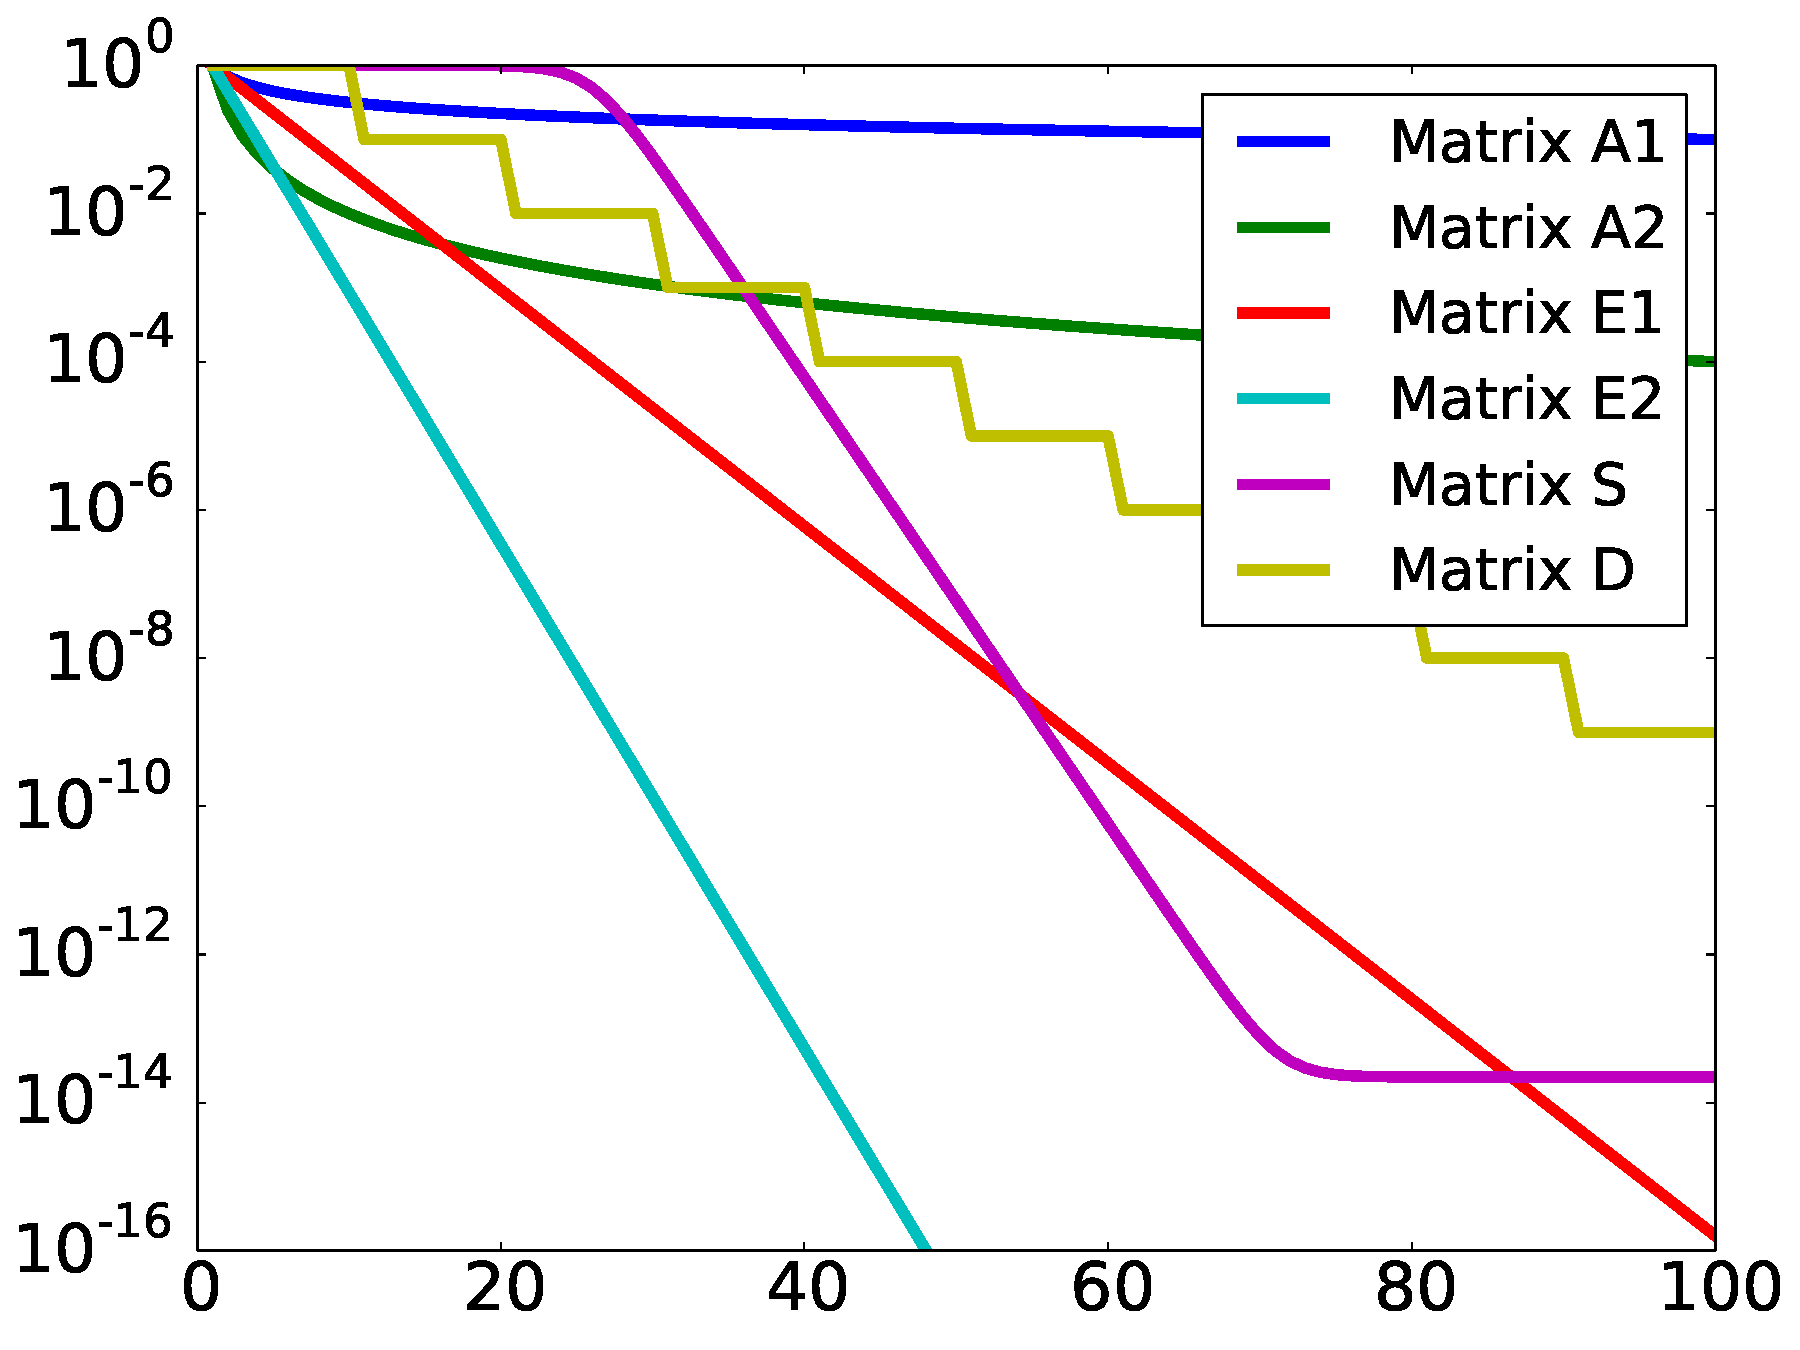
\includegraphics[width=8cm]{plots/sing_value_plot_dis.pdf}
\caption[Matrix Singular Values]{
A plot of the singular values for the matrices we
are investigating.}
\label{fig:sing_decay}
\end{figure}


\subsection{Norm Approximation}
% Give examples to show how HMT over estimates norm

We begin by showing how poorly the HMT error bound from
Lem.~\ref{thm:rand_hmt_bound} is by using it to estimate
$\norm{A}_{2}$; the results are shown
in Table~\ref{tab:hmt_norm_ubound_mat}, and we remember $\norm{A}_{2}\approx1$.
We let $\alpha\in\braces{2,5,10}$ and choose the number of samples
$p$ so that $\alpha^{p}\le 10^{-\ell}$ for various $\ell$.
To allow for comparisons, we let
$\alpha^{p}\in\braces{10^{-9},10^{-12},10^{-15}}$.
It is clear that in \emph{every} case the norm is overestimated, always
$3\times$ and frequently $10\times$ larger; furthermore, smaller $\alpha$
always leads to a more accurate estimate.
As we can see, we greatly overestimate the norm.
We are able to accurately measure the F-norm as seen
in Fig.~\ref{fig:geb_norm_bound_mat} using our stochastic estimate;
note the logarithmic scale on the number of columns ($d$).
We also include estimates of the squared F-norm in
Fig.~\ref{fig:geb_norm_squared_bound_mat} including mean and standard
deviations as well as the theoretical standard deviations;
the predicted results accurately match expected results.
We averaged 10,000 trials to obtain the statistics for these results.
In order to obtain the theoretical standard deviations in
Fig.~\ref{fig:geb_norm_squared_bound_mat}, we took the square root
of the variance from Eq.~\eqref{eq:rand_Xd_variance_bounds}.

%%%%%%%%%%%%%%%%%%%%%%%%%%%%%%%%%%%%%%%%%%%%%%%%%%%%%%%%%%%%%%%%%%%%%%%%
%%% Table of Upper Bounds for 2-Norm estimates

\begin{table}
\begin{center}
\begin{tabular}{cc|c|c|c|c|c|c|c|c|c|}
\cline{3-11}
& & \multicolumn{3}{|c|}{\textbf{1E-9}} &
\multicolumn{3}{|c|}{\textbf{1E-12}} & \multicolumn{3}{|c|}{\textbf{1E-15}} \\
\cline{3-11}
& & $p$ & M & S & $p$ & M & S & $p$ & M & S \\
\hline
\multicolumn{1}{|c|}{\multirow{3}{*}{Matrix A1}} & \textbf{2} &
    30 & 5.11 & 0.53 & 40 & 5.23 & 0.52 & 50 & 5.32 & 0.52 \\
\cline{2-11}
\multicolumn{1}{|c|}{} &\textbf{5} &
    13 & 11.8 & 1.4 & 18 & 12.2 & 1.4 & 22 & 12.4 & 1.3 \\
\cline{2-11}
\multicolumn{1}{|c|}{} &\textbf{10} &
    9 & 22.9 & 2.8  & 12 & 23.5 & 2.8  & 15 & 24.1 & 2.7 \\
\hline
\hline
\multicolumn{1}{|c|}{\multirow{3}{*}{Matrix A2}} & \textbf{2} &
    30 & 3.73 & 0.71 & 40 & 3.90 & 0.69 & 50 & 4.03 & 0.68 \\
\cline{2-11}
\multicolumn{1}{|c|}{} & \textbf{5} &
    13 & 8.02 & 1.93 & 18 & 8.52 & 1.86 & 22 & 8.85 & 1.82 \\
\cline{2-11}
\multicolumn{1}{|c|}{} & \textbf{10} &
    9 & 14.8 & 4.0  & 12 & 15.8 & 3.9  & 15 & 16.5 & 3.8 \\
\hline
\hline
\multicolumn{1}{|c|}{\multirow{3}{*}{Matrix E1}} & \textbf{2} &
    30 & 4.11 & 0.64 & 40 & 4.26 & 0.63 & 50 & 4.38 & 0.62 \\
\cline{2-11}
\multicolumn{1}{|c|}{} & \textbf{5} &
    13 & 9.14  & 1.72  & 18 & 9.58  & 1.68  & 22 & 9.86  & 1.66 \\
\cline{2-11}
\multicolumn{1}{|c|}{} & \textbf{10} &
    9 & 17.2 & 3.6   & 12 & 18.0  & 3.5  & 15 & 18.7 & 3.4 \\
\hline
\hline
\multicolumn{1}{|c|}{\multirow{3}{*}{Matrix E2}} & \textbf{2} &
    30 & 3.81 & 0.70 & 40 & 3.98 & 0.68 & 50 & 4.10 & 0.67 \\
\cline{2-11}
\multicolumn{1}{|c|}{} & \textbf{5} &
    13 & 8.27  & 1.90  & 18 & 8.78  & 1.83  & 22 & 9.07  & 1.79 \\
\cline{2-11}
\multicolumn{1}{|c|}{} & \textbf{10} &
    9 & 15.3 & 3.94   & 12 & 16.3  & 3.84  & 15 & 17.0 & 3.74 \\
\hline
\hline
\multicolumn{1}{|c|}{\multirow{3}{*}{Matrix S}} & \textbf{2} &
    30 & 10.1 & 0.6 & 40 & 10.2 & 0.6 & 50 & 10.3 & 0.6 \\
\cline{2-11}
\multicolumn{1}{|c|}{} & \textbf{5} &
    13 & 24.1  & 1.6  & 18 & 24.5  & 1.6  & 22 & 24.8  & 1.5 \\
\cline{2-11}
\multicolumn{1}{|c|}{} & \textbf{10} &
    9 & 47.0 & 3.5   & 12 & 47.9  & 3.3  & 15 & 48.5 & 3.2 \\
\hline
\hline
\multicolumn{1}{|c|}{\multirow{3}{*}{Matrix D}} & \textbf{2} &
    30 & 7.36 & 0.64 & 40 & 7.51 & 0.61 & 50 & 7.61 & 0.60 \\
\cline{2-11}
\multicolumn{1}{|c|}{} & \textbf{5} &
    13 & 17.2  & 1.8  & 18 & 17.7  & 1.7  & 22 & 18.0  & 1.6 \\
\cline{2-11}
\multicolumn{1}{|c|}{} & \textbf{10} &
    9 & 33.3 & 3.7   & 12 & 34.2  & 3.6  & 15 & 34.8 & 3.5 \\
\hline
\end{tabular}
\end{center}
\caption[HMT 2-Norm Upper Bounds]{
Upper bound of $||A||_{2}$ based on
 Lemma~\ref{thm:rand_hmt_bound} (HMT) for different
failure probabilities (columns) and $\alpha$ (rows).
$p$ is the smallest integer for which $\alpha^{-p}\le 10^{-\ell}$.
We performed 10,000 trials and computed the mean (M) and standard deviation
(S). The correct values are $||A||_{2}\approx1$.
}
\label{tab:hmt_norm_ubound_mat}
\end{table}

% Print results for GEB estimates for F-norm

\begin{figure}[p]
    \centering

    \begin{subfigure}{0.45\textwidth}
    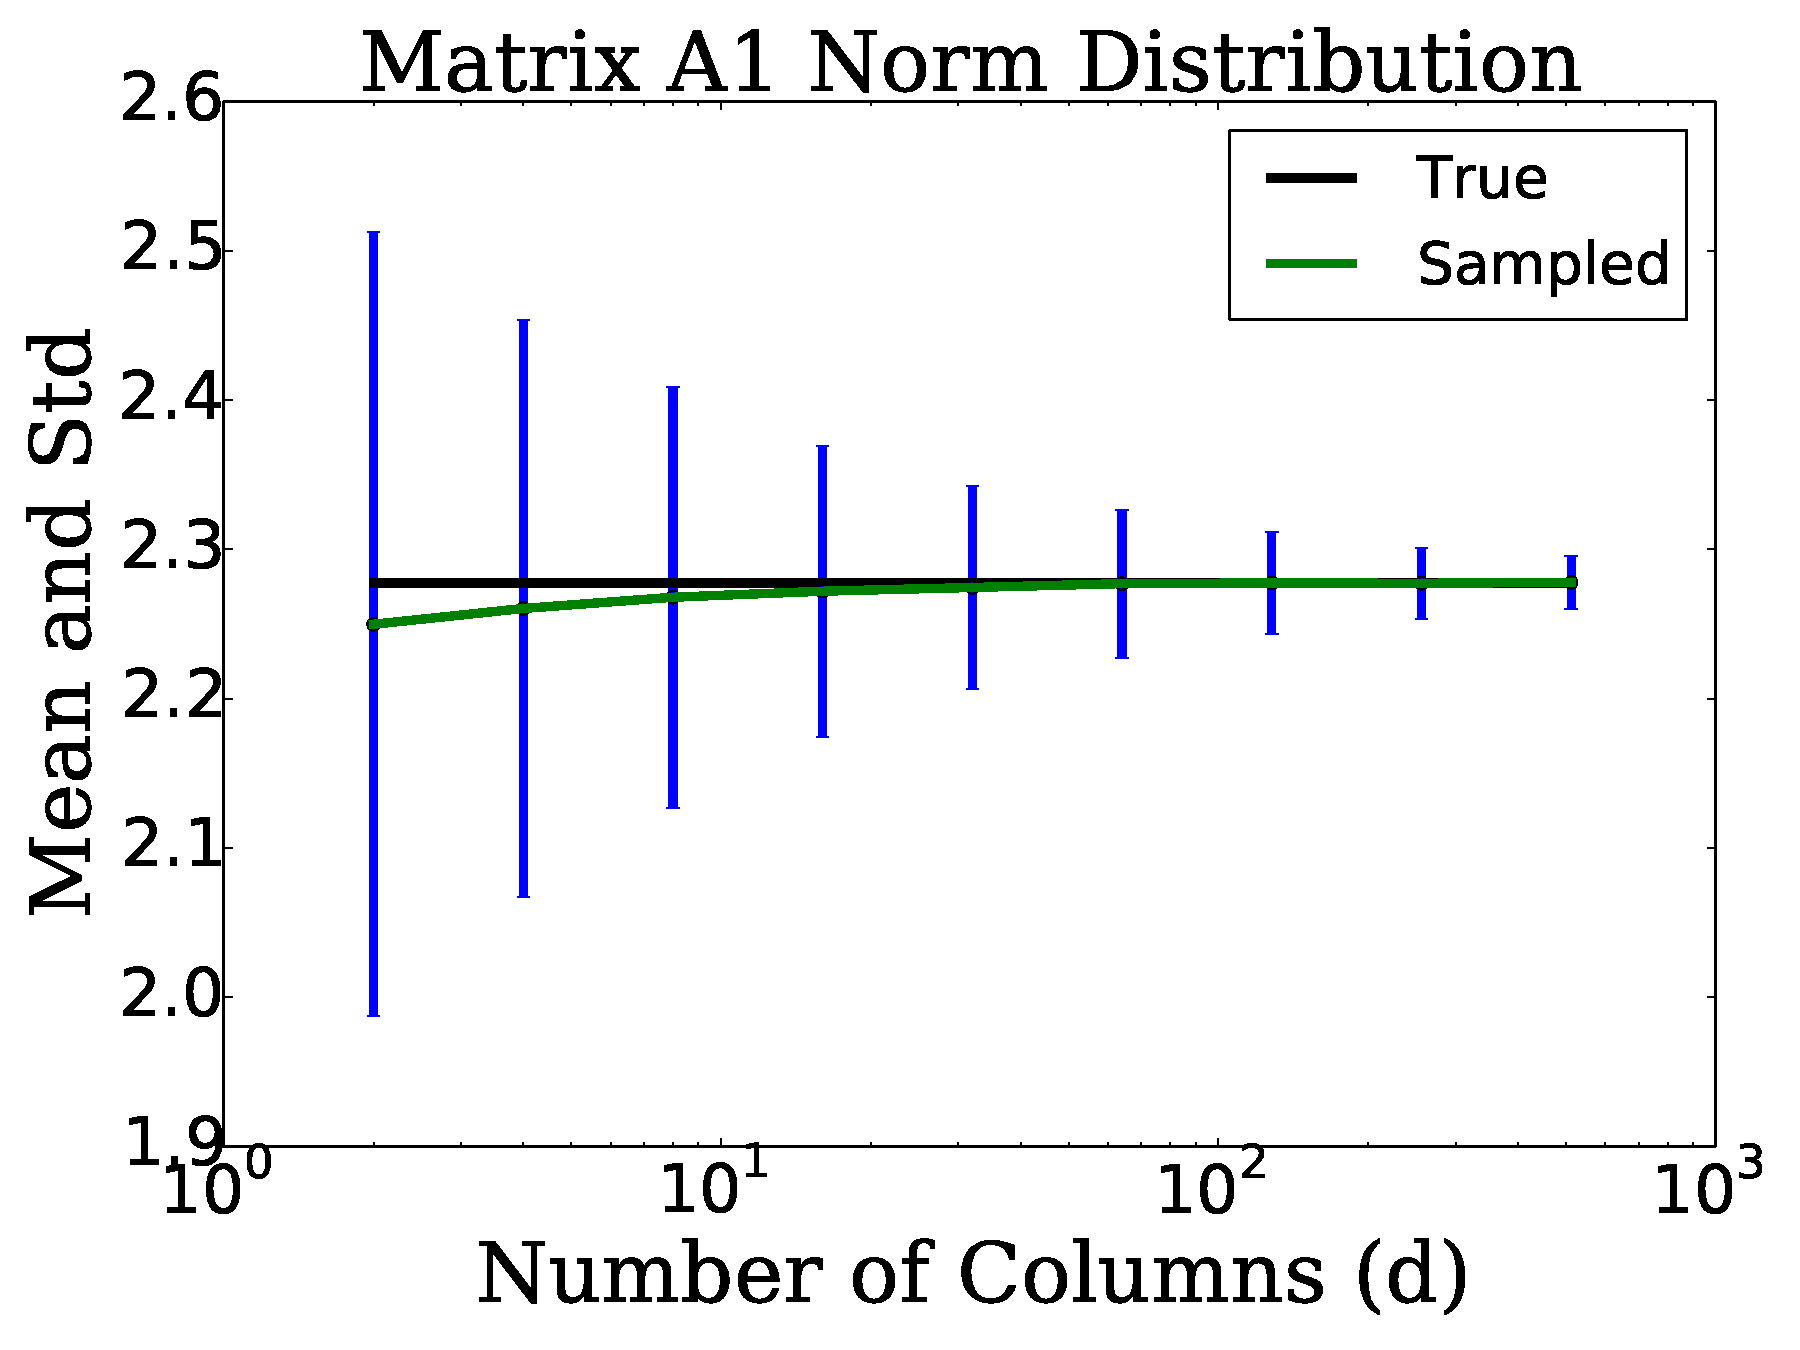
\includegraphics[width=\textwidth]{plots/mat_A1_error_test.pdf}
    \caption{Matrix A1}
    \end{subfigure}
    \begin{subfigure}{0.45\textwidth}
    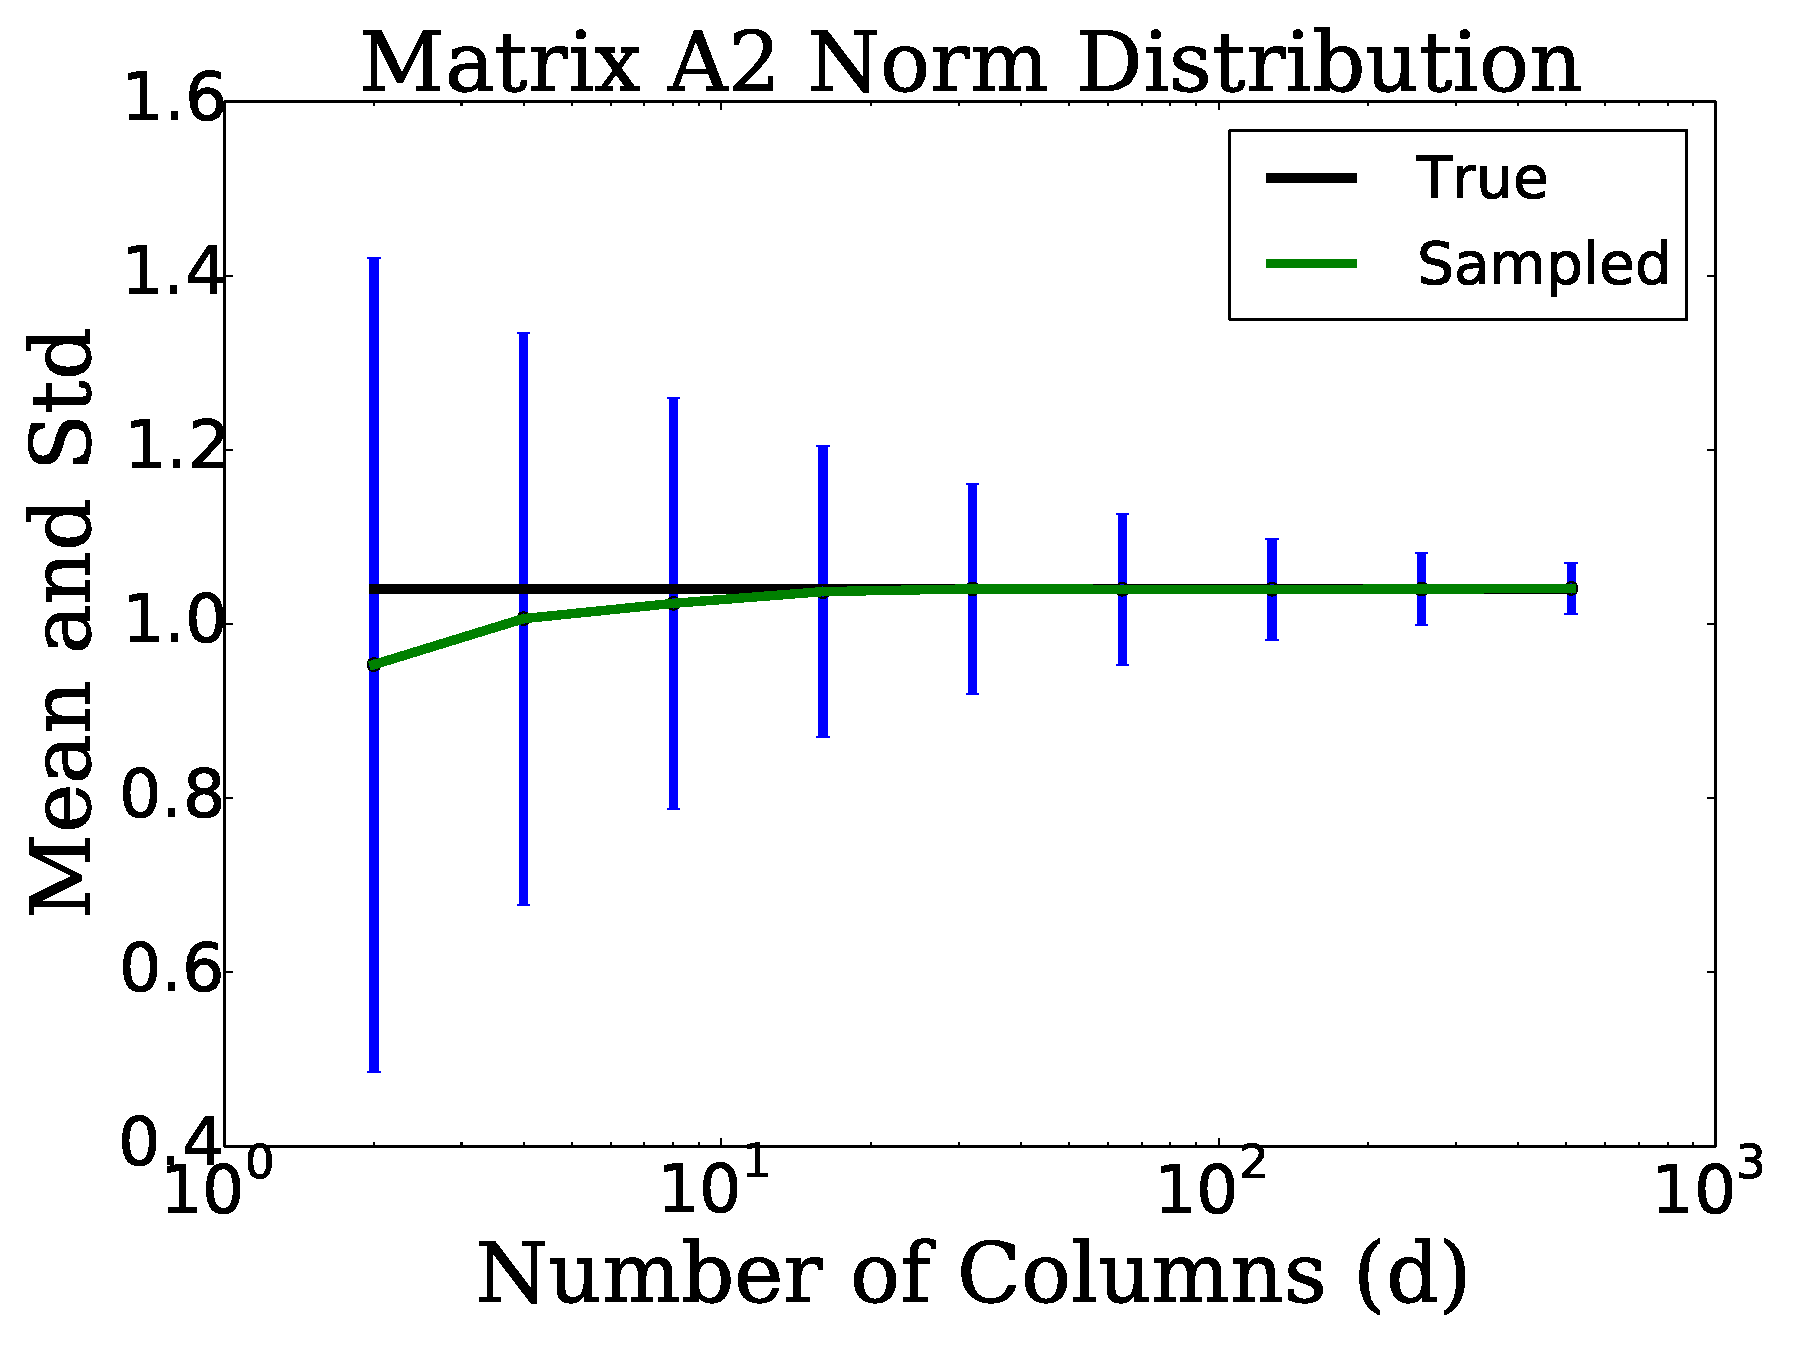
\includegraphics[width=\textwidth]{plots/mat_A2_error_test.pdf}
    \caption{Matrix A2}
    \end{subfigure}

    \begin{subfigure}{0.45\textwidth}
    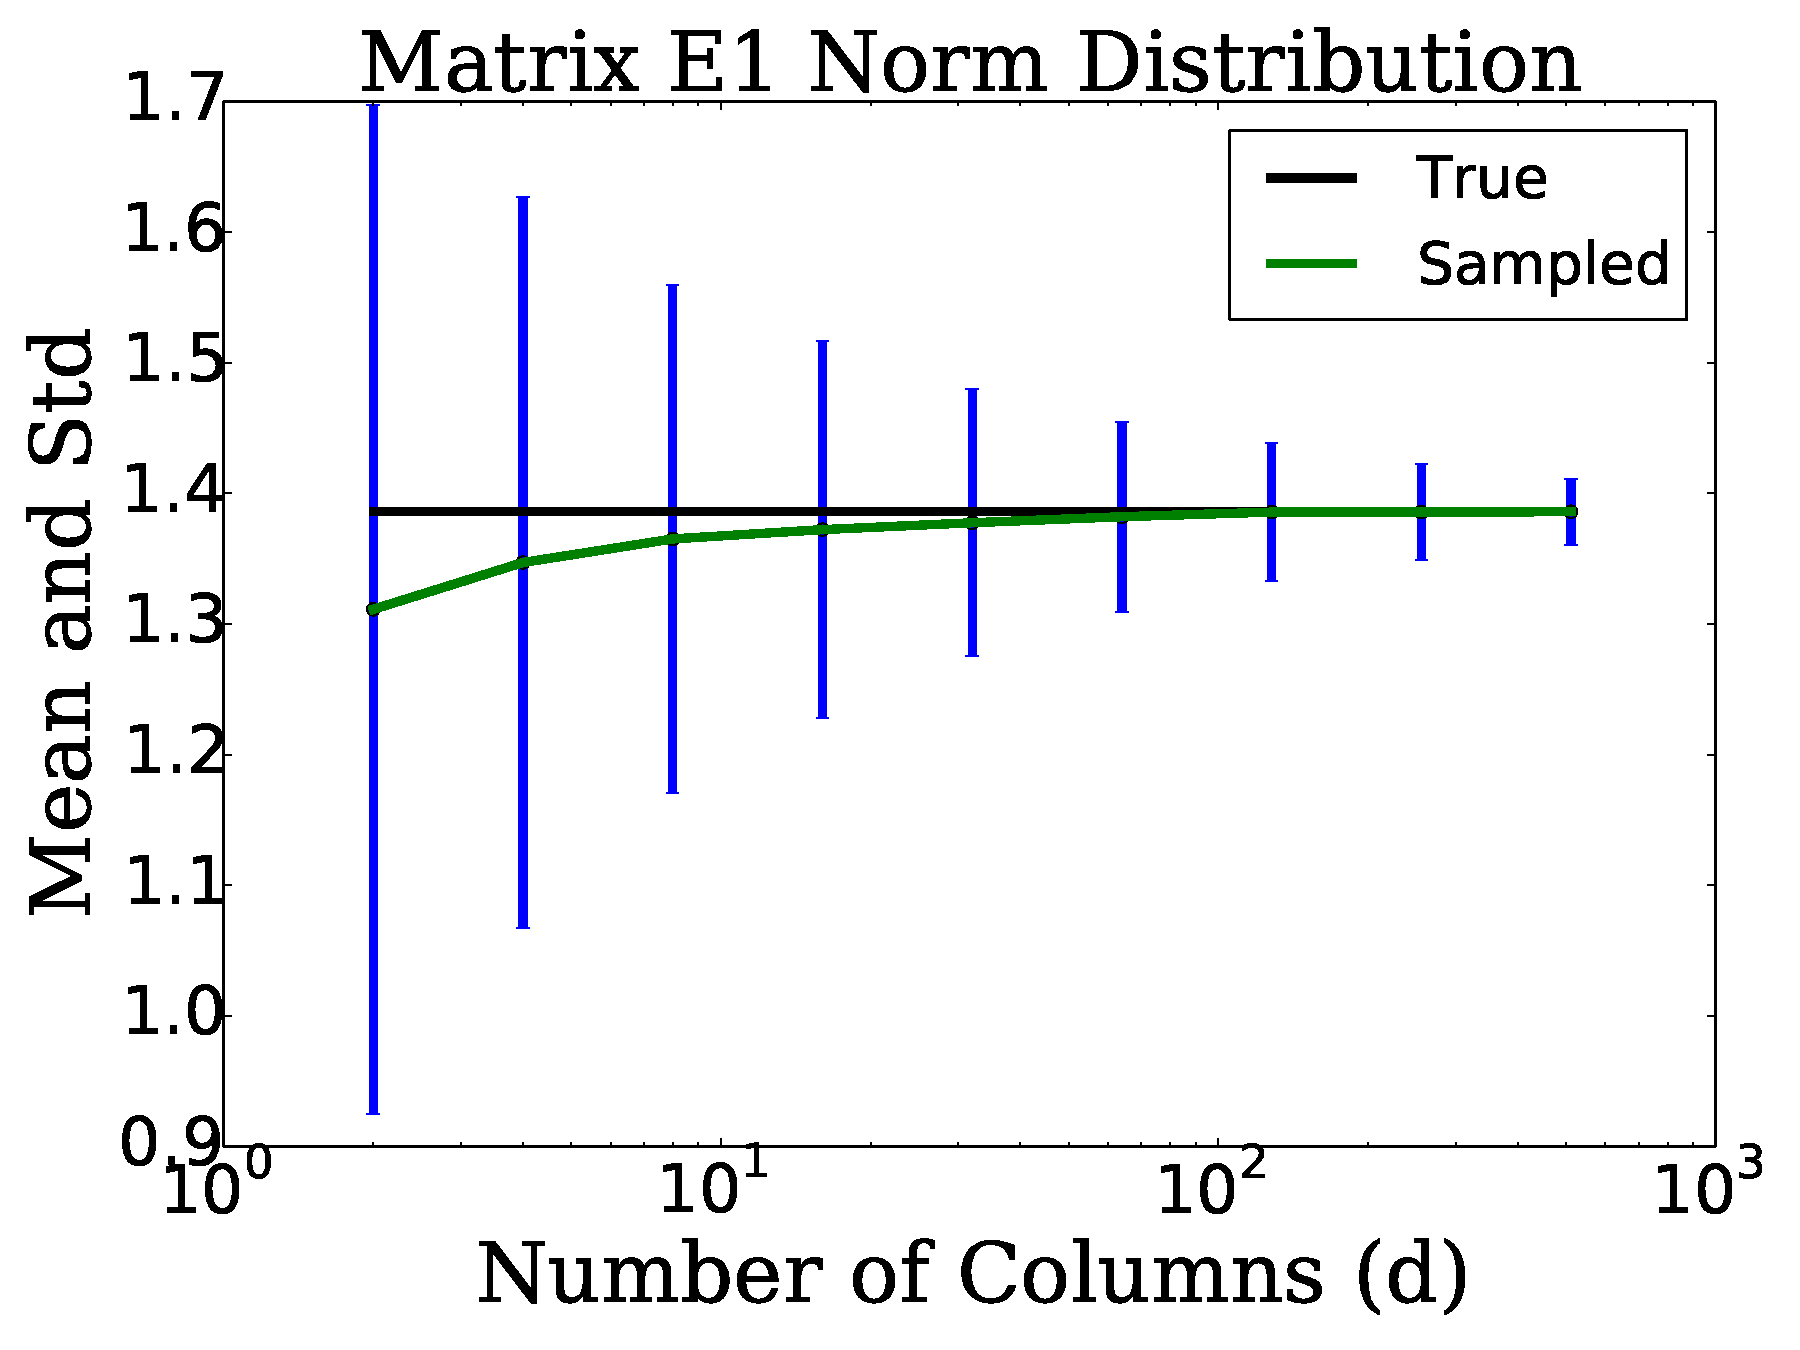
\includegraphics[width=\textwidth]{plots/mat_E1_error_test.pdf}
    \caption{Matrix E1}
    \end{subfigure}
    \begin{subfigure}{0.45\textwidth}
    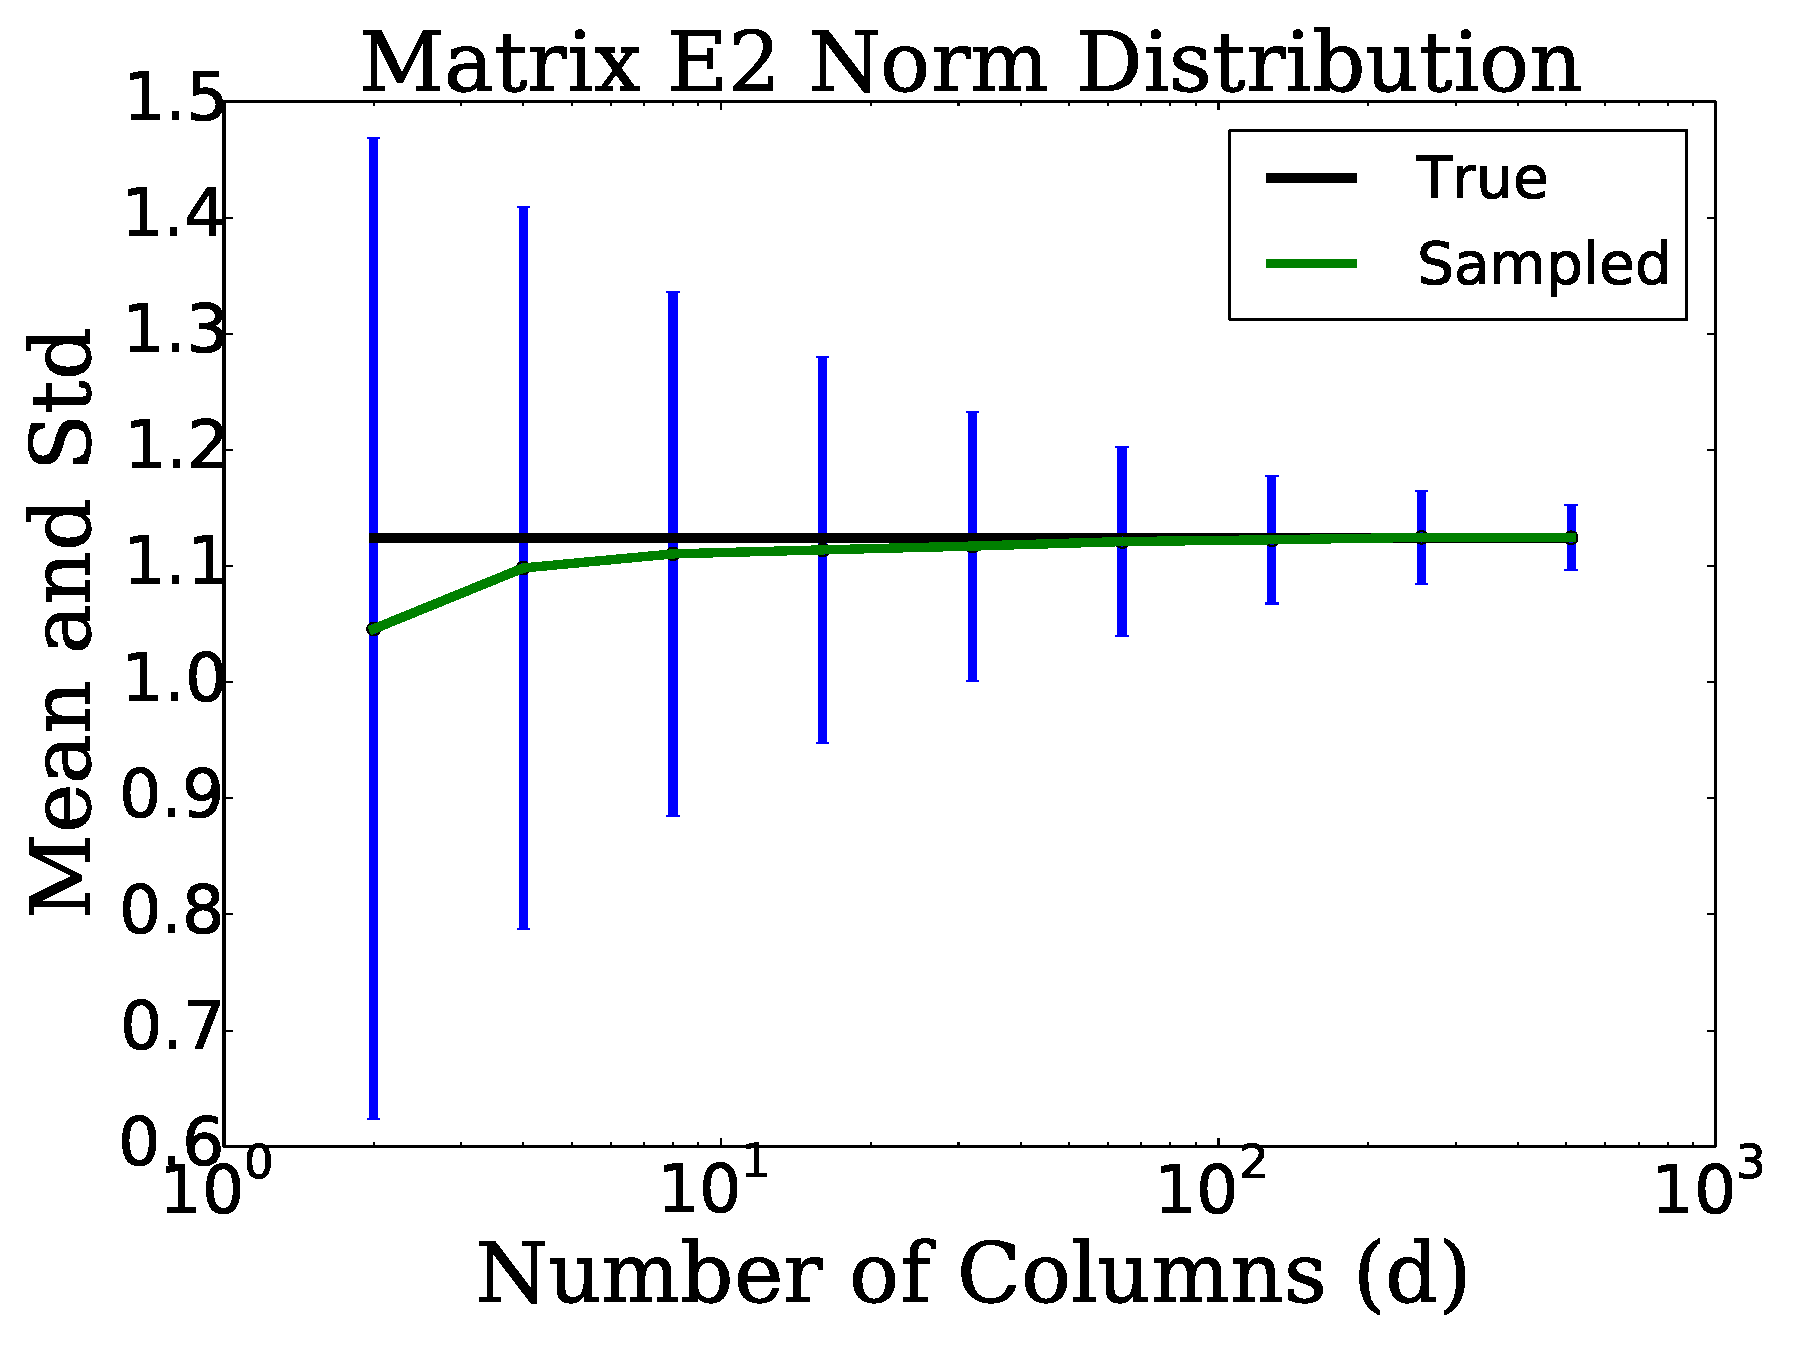
\includegraphics[width=\textwidth]{plots/mat_E2_error_test.pdf}
    \caption{Matrix E2}
    \end{subfigure}

    \begin{subfigure}{0.45\textwidth}
    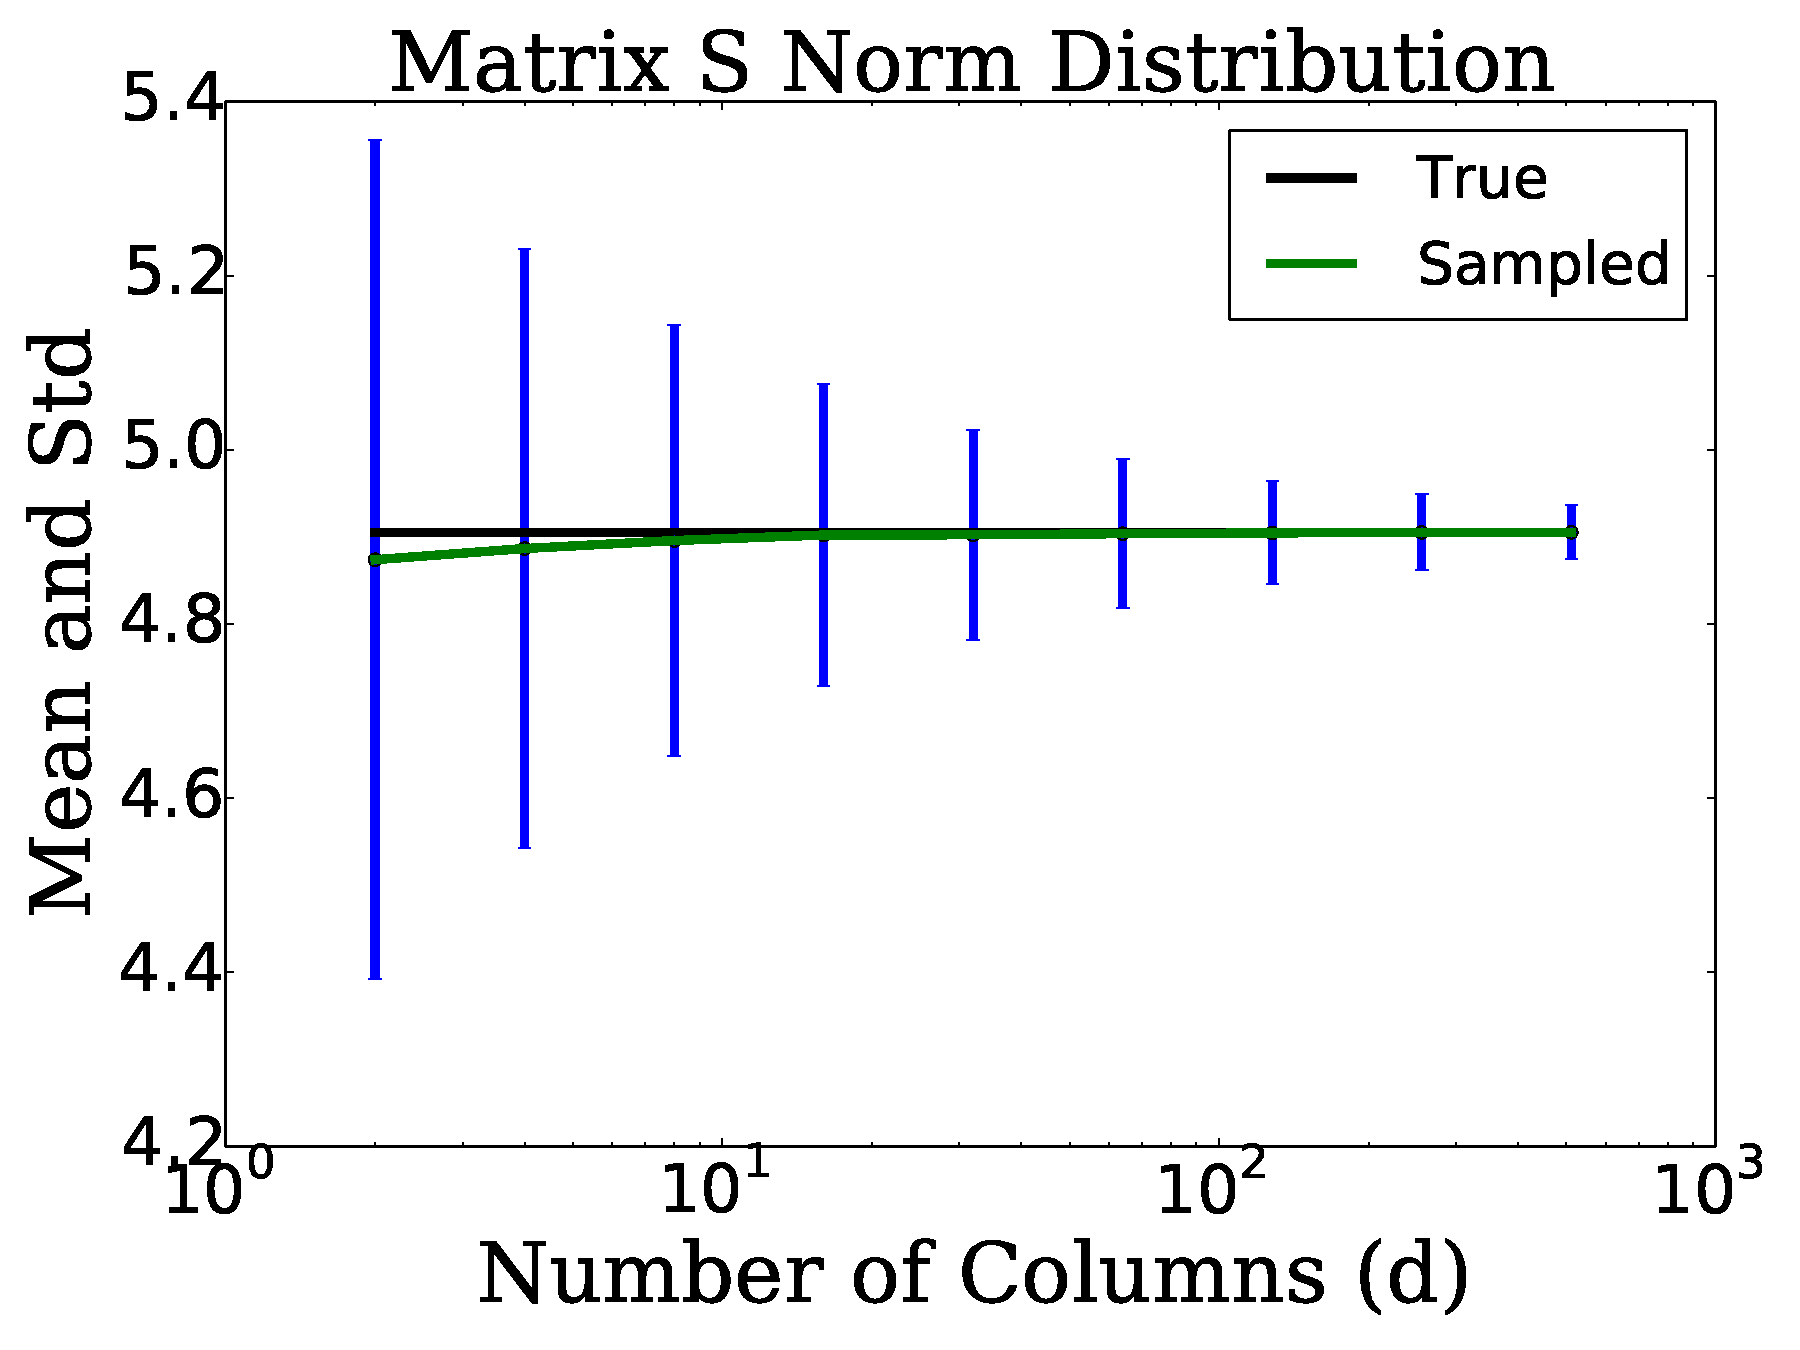
\includegraphics[width=\textwidth]{plots/mat_S_error_test.pdf}
    \caption{Matrix S}
    \end{subfigure}
    \begin{subfigure}{0.45\textwidth}
    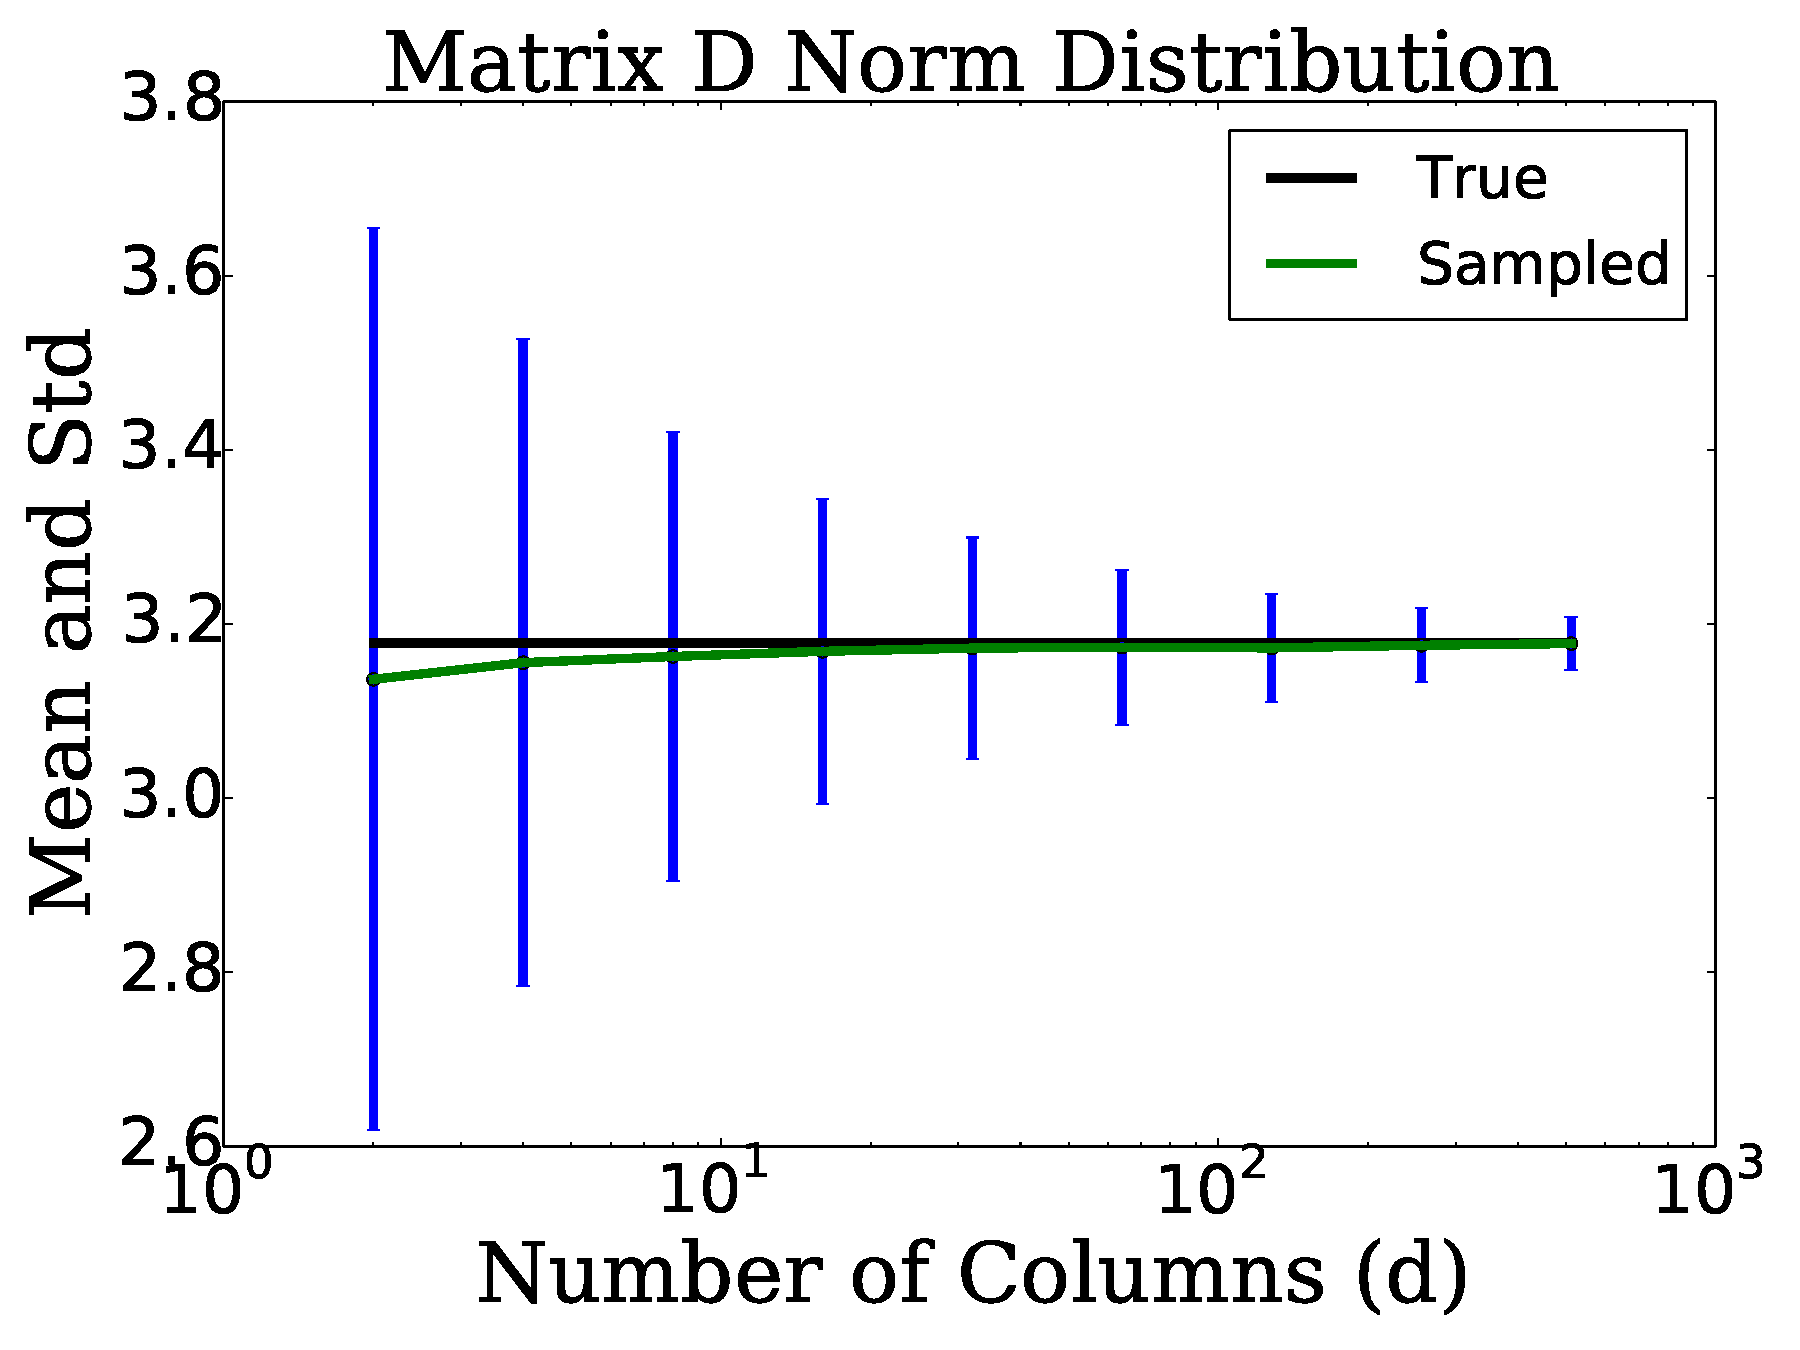
\includegraphics[width=\textwidth]{plots/mat_D_error_test.pdf}
    \caption{Matrix D}
    \end{subfigure}

\caption[GEB Stochastic F-norm Approximations]{
%Estimated $||A||_{F}$ for our matrices using the Gaussian Error Bound.
We performed 10,000 trials and computed the mean (Green) and
standard deviation (Blue) of $\norm{A\Omega}_{F}$ for columns
$d\in\{2,4,8,\cdots,512\}$.
The true F-norm value is Black.
}
\label{fig:geb_norm_bound_mat}
\end{figure}




% Print results for GEB estimates for F-norm^2

\begin{figure}[p]
    \centering

    \begin{subfigure}{0.45\textwidth}
    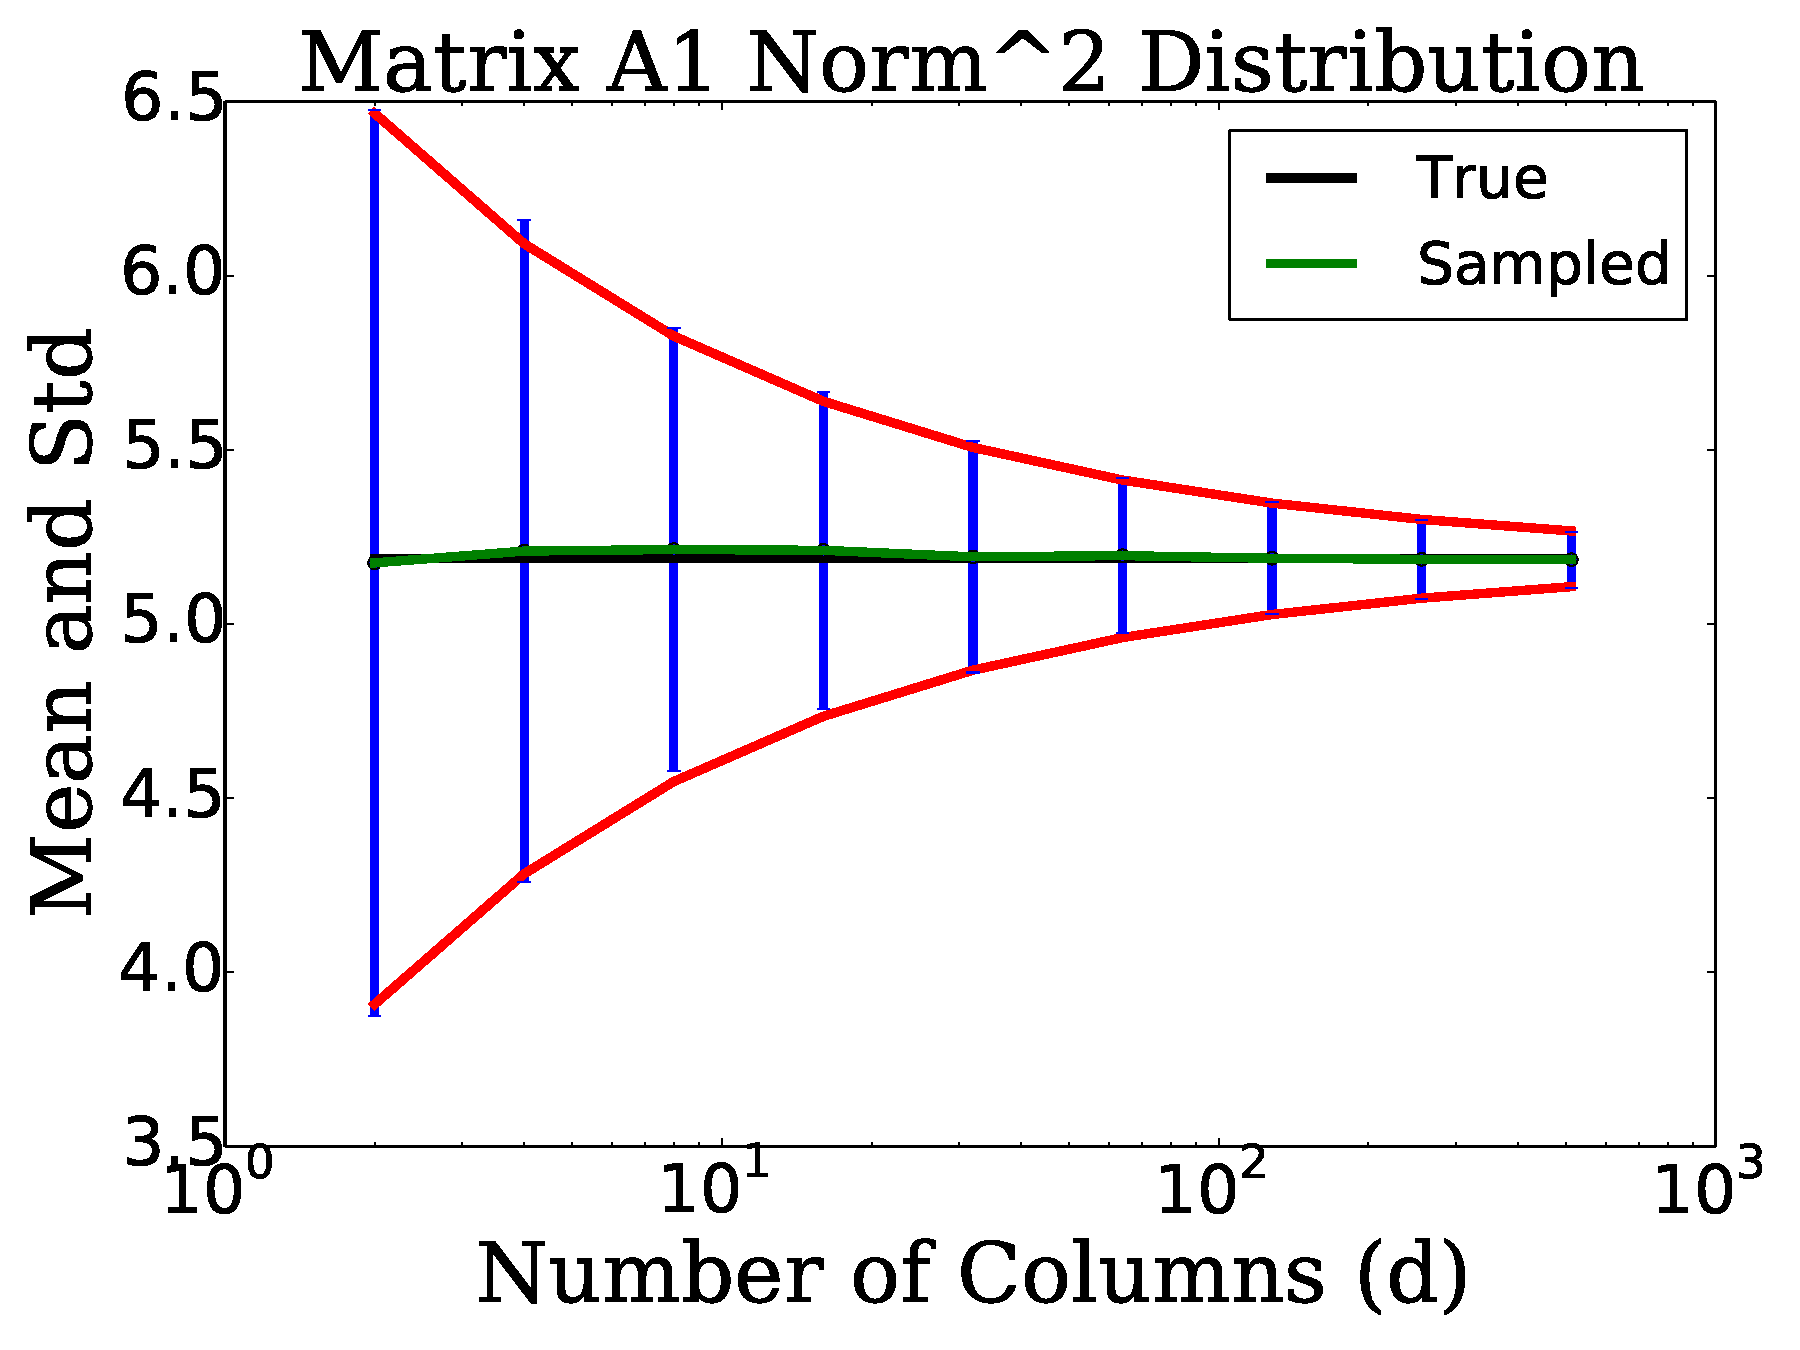
\includegraphics[width=\textwidth]{plots/mat_A1_error_test_2.pdf}
    \caption{Matrix A1}
    \end{subfigure}
    \begin{subfigure}{0.45\textwidth}
    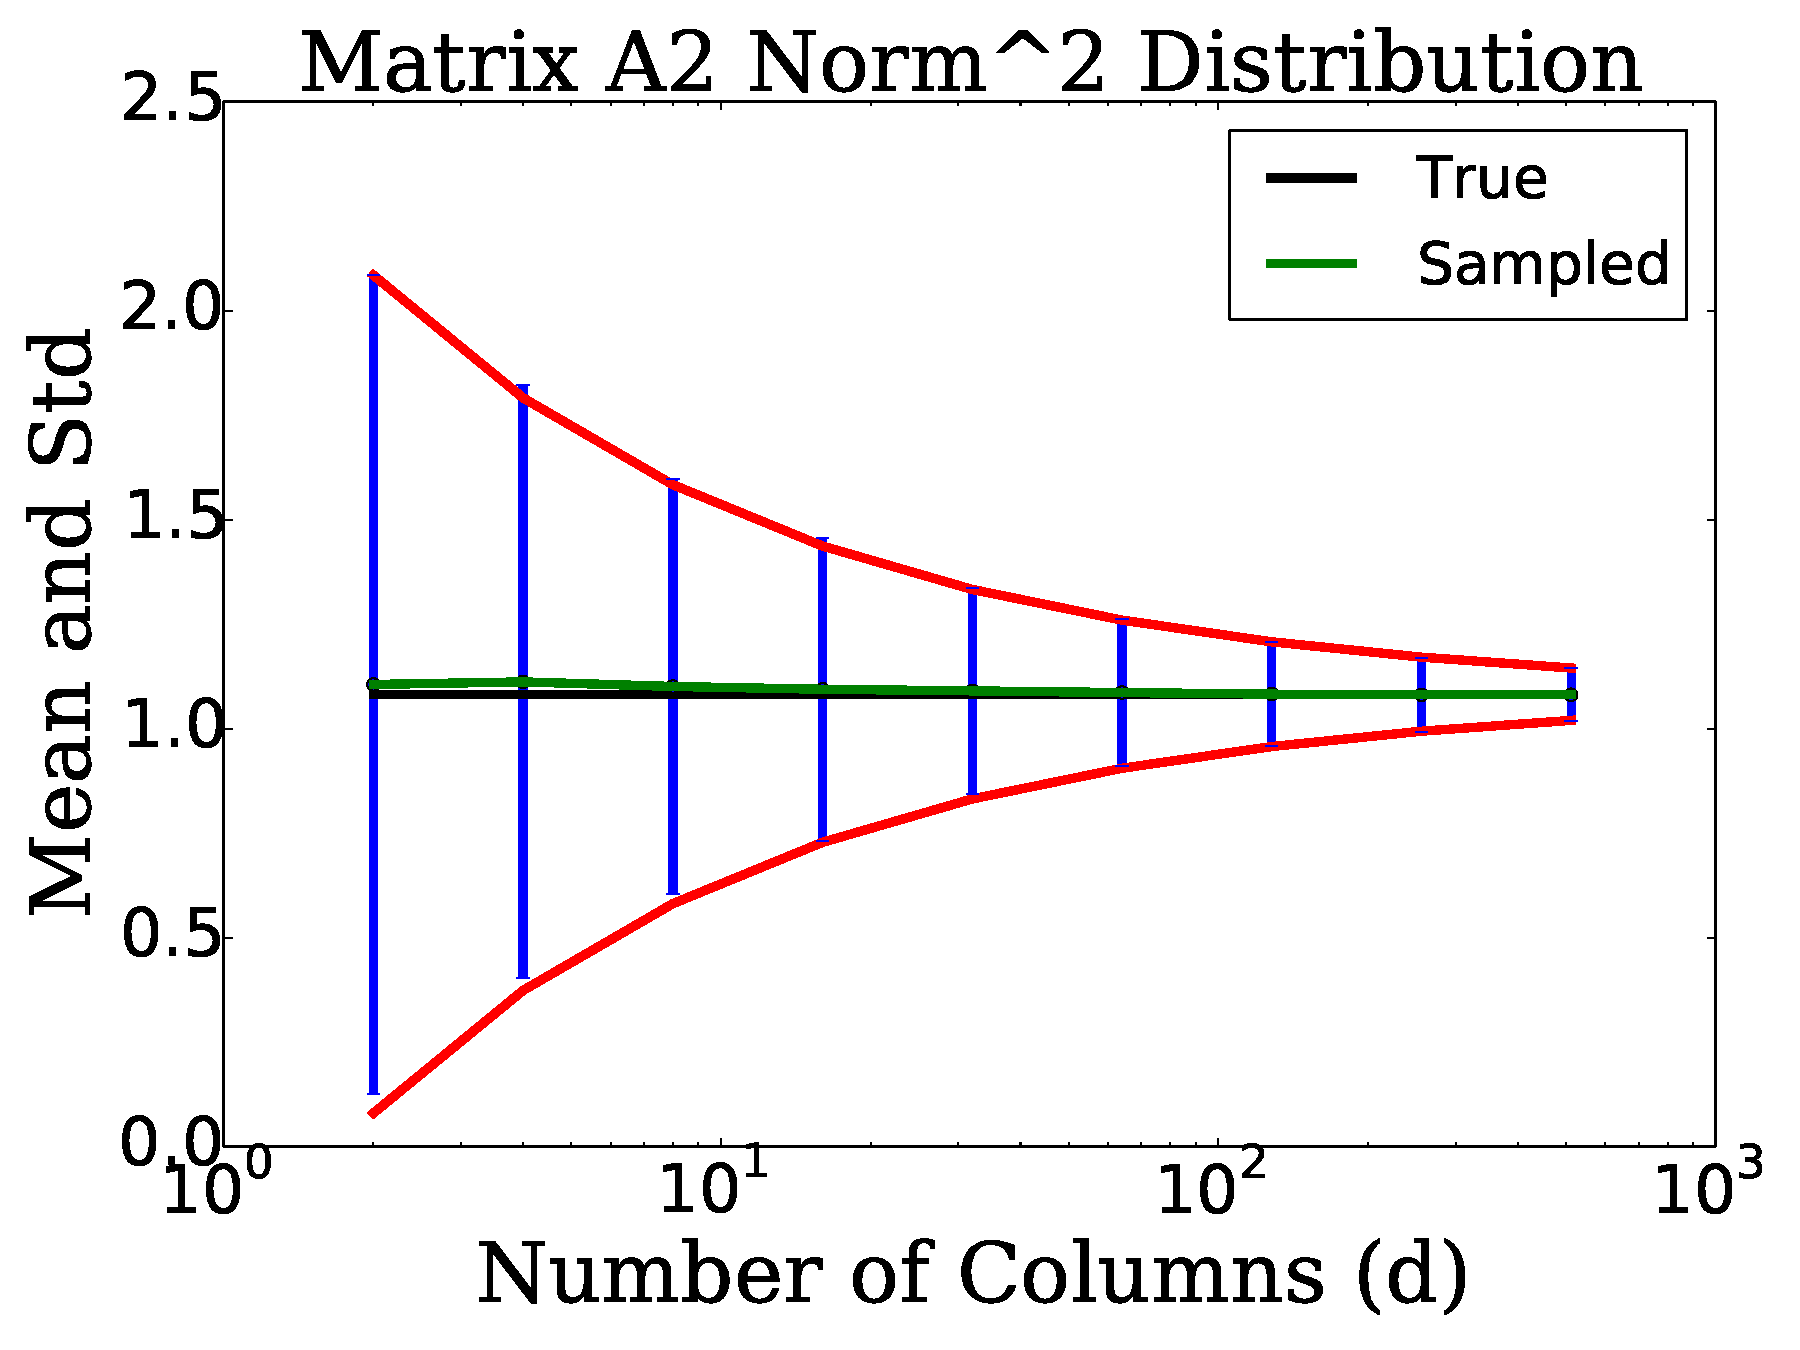
\includegraphics[width=\textwidth]{plots/mat_A2_error_test_2.pdf}
    \caption{Matrix A2}
    \end{subfigure}

    \begin{subfigure}{0.45\textwidth}
    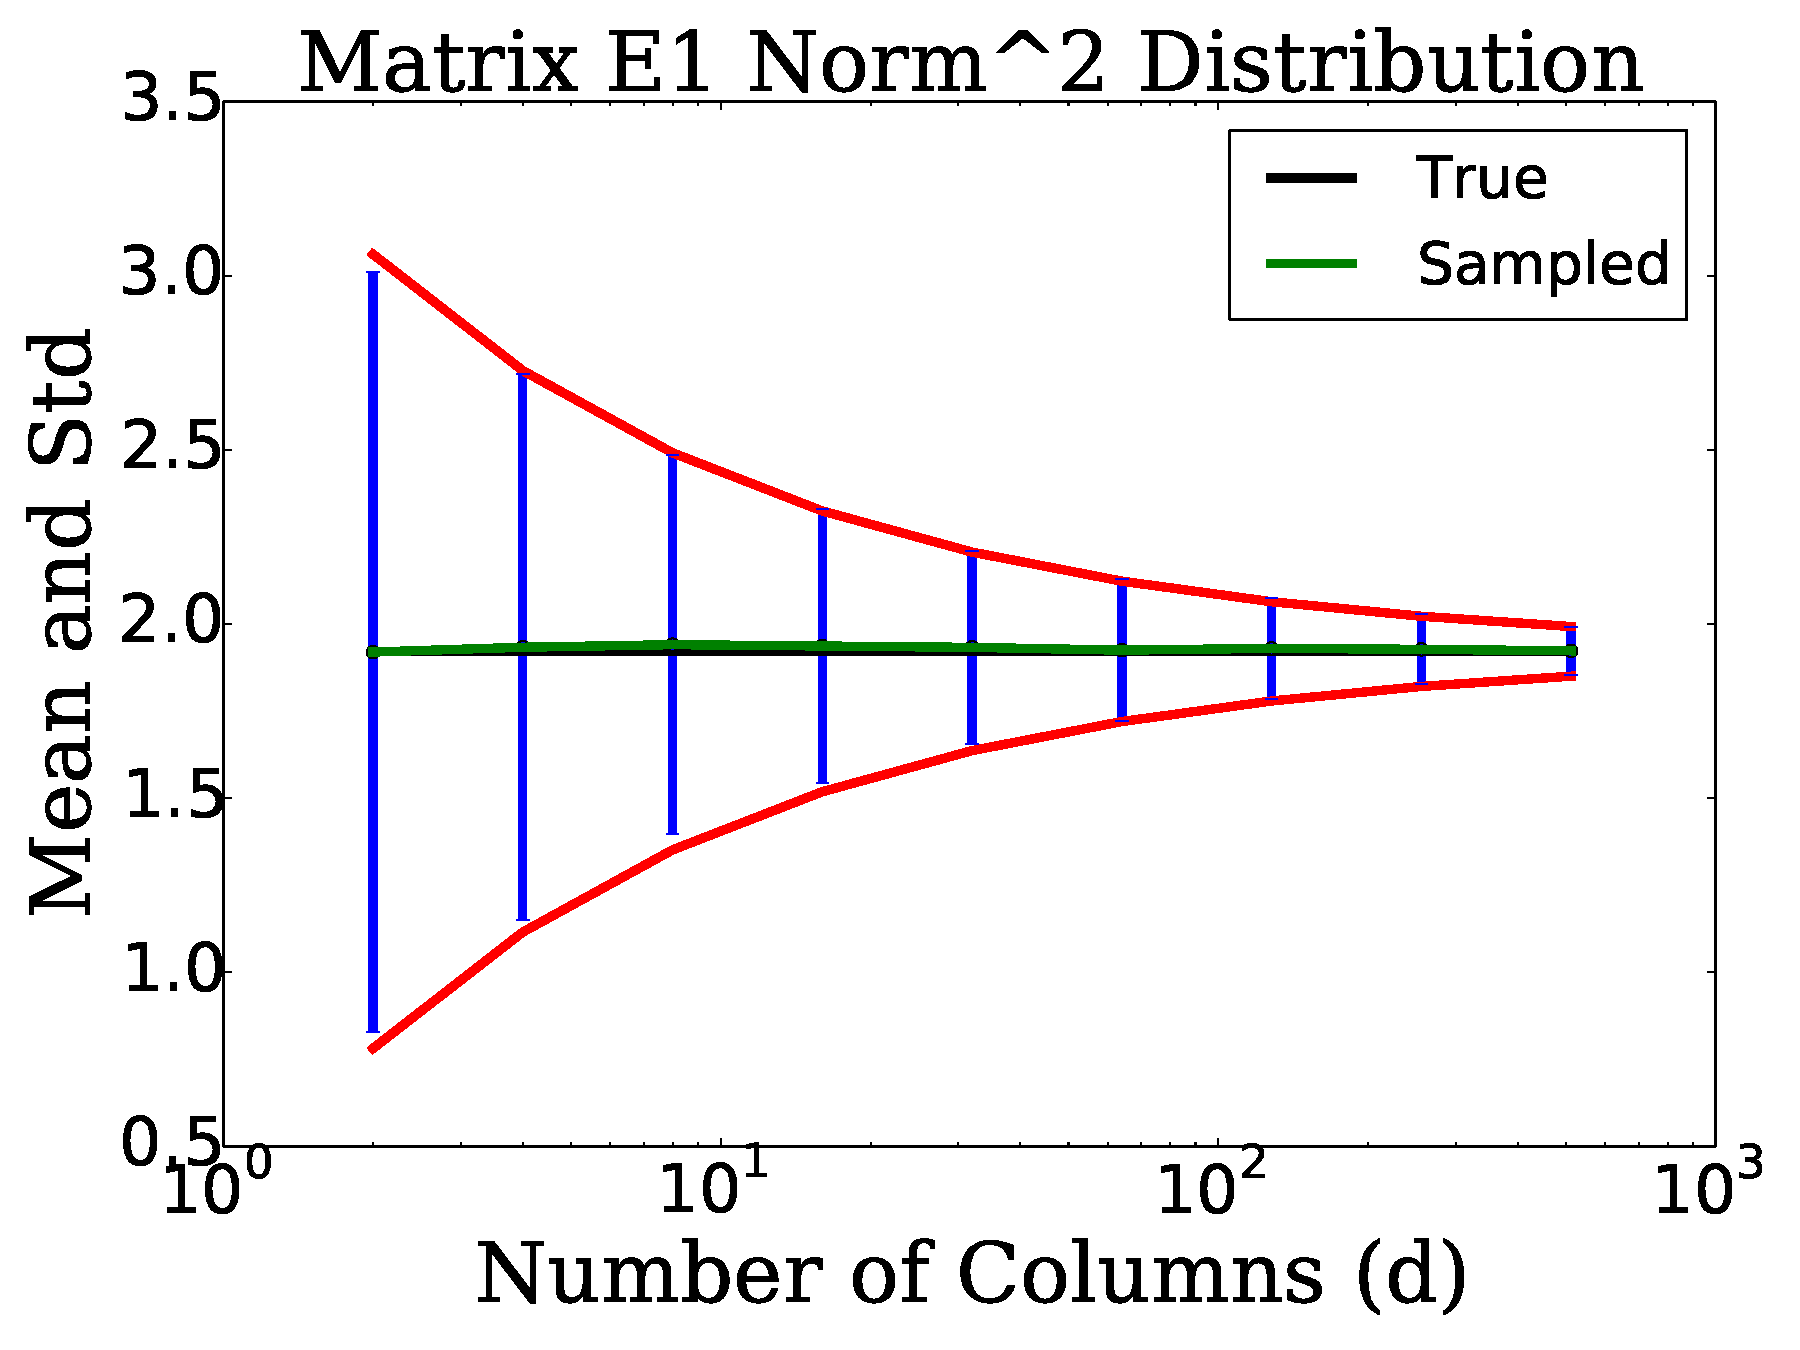
\includegraphics[width=\textwidth]{plots/mat_E1_error_test_2.pdf}
    \caption{Matrix E1}
    \end{subfigure}
    \begin{subfigure}{0.45\textwidth}
    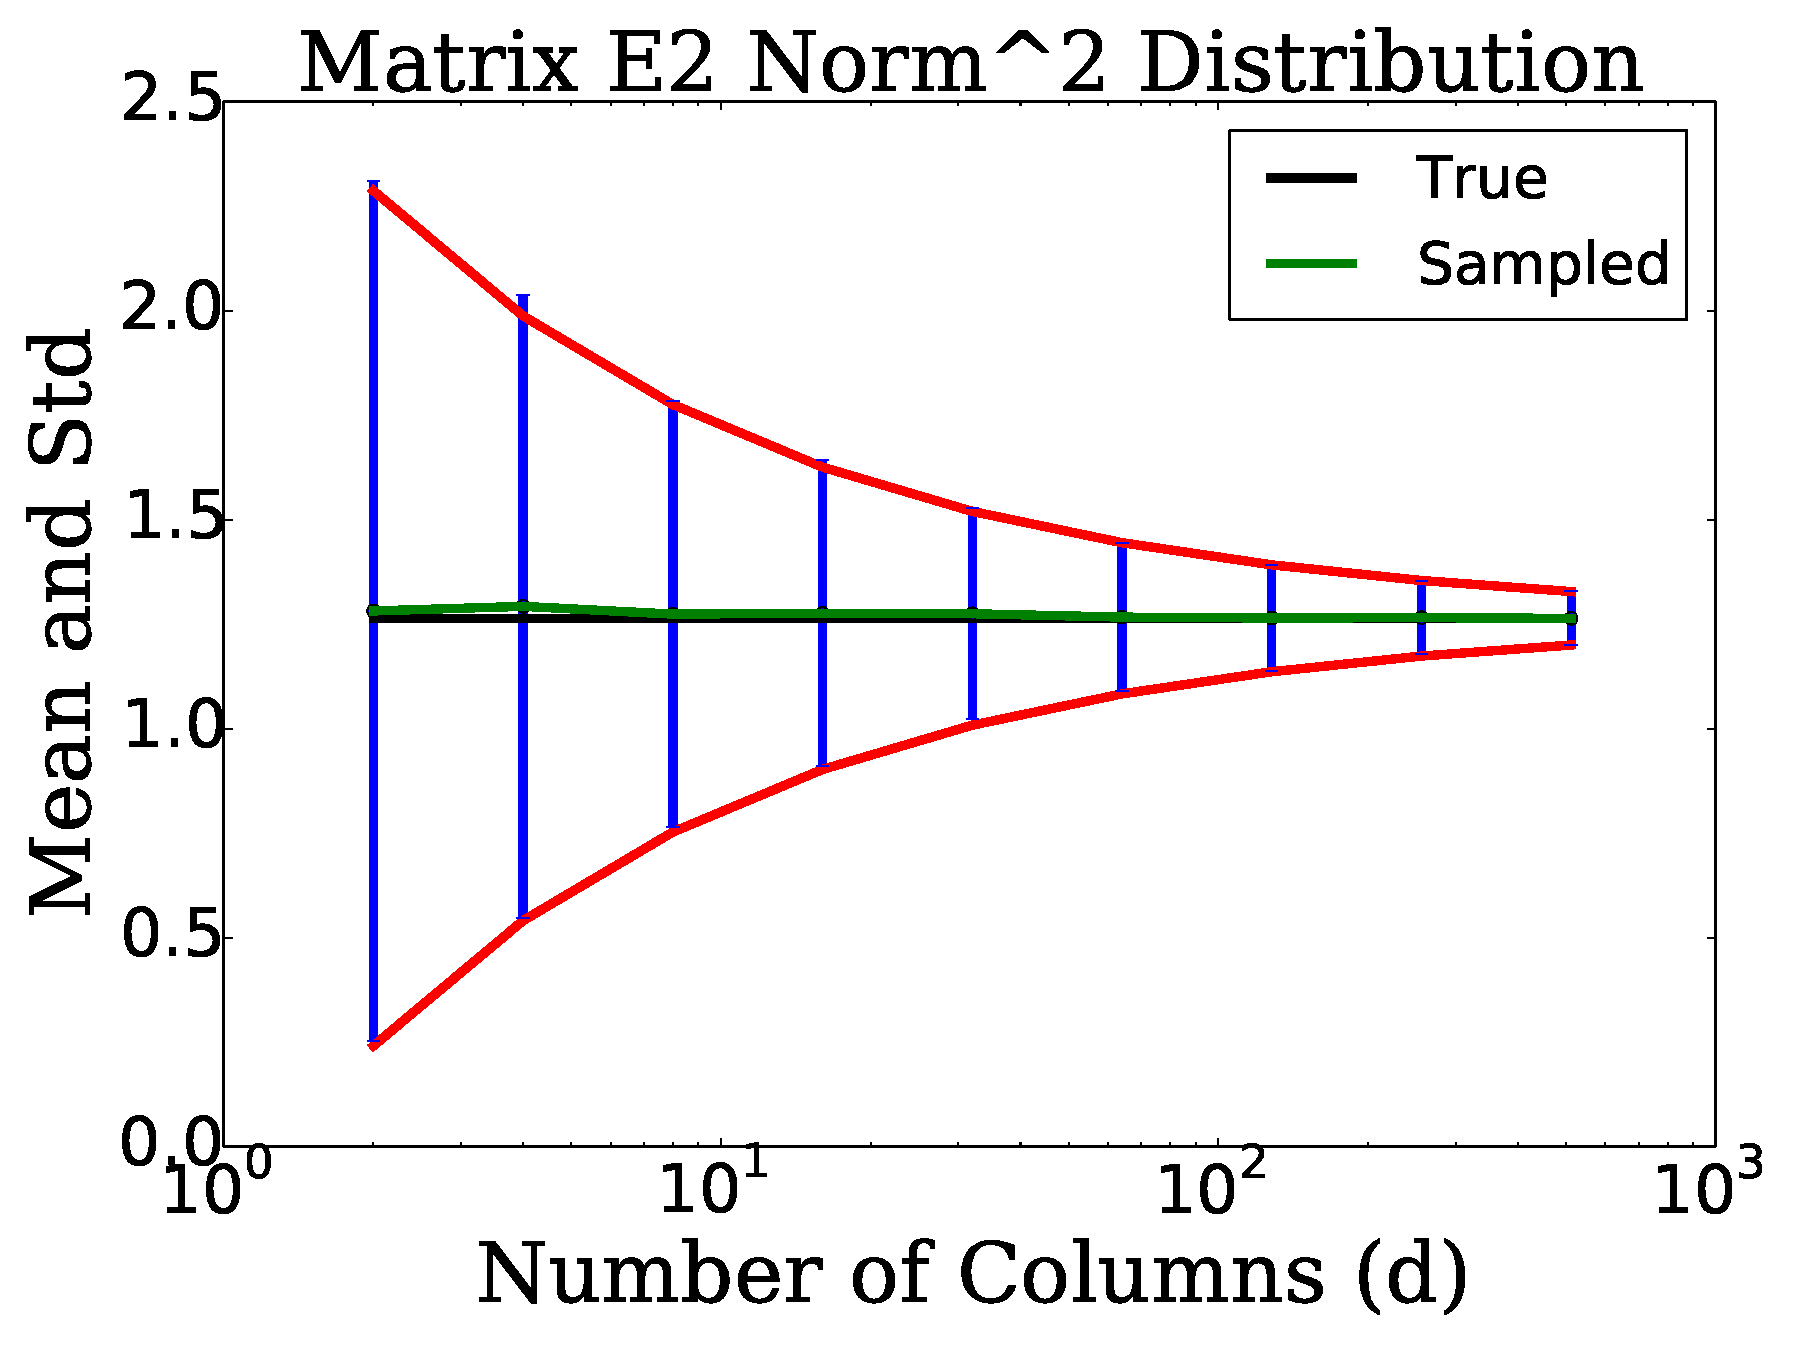
\includegraphics[width=\textwidth]{plots/mat_E2_error_test_2.pdf}
    \caption{Matrix E2}
    \end{subfigure}

    \begin{subfigure}{0.45\textwidth}
    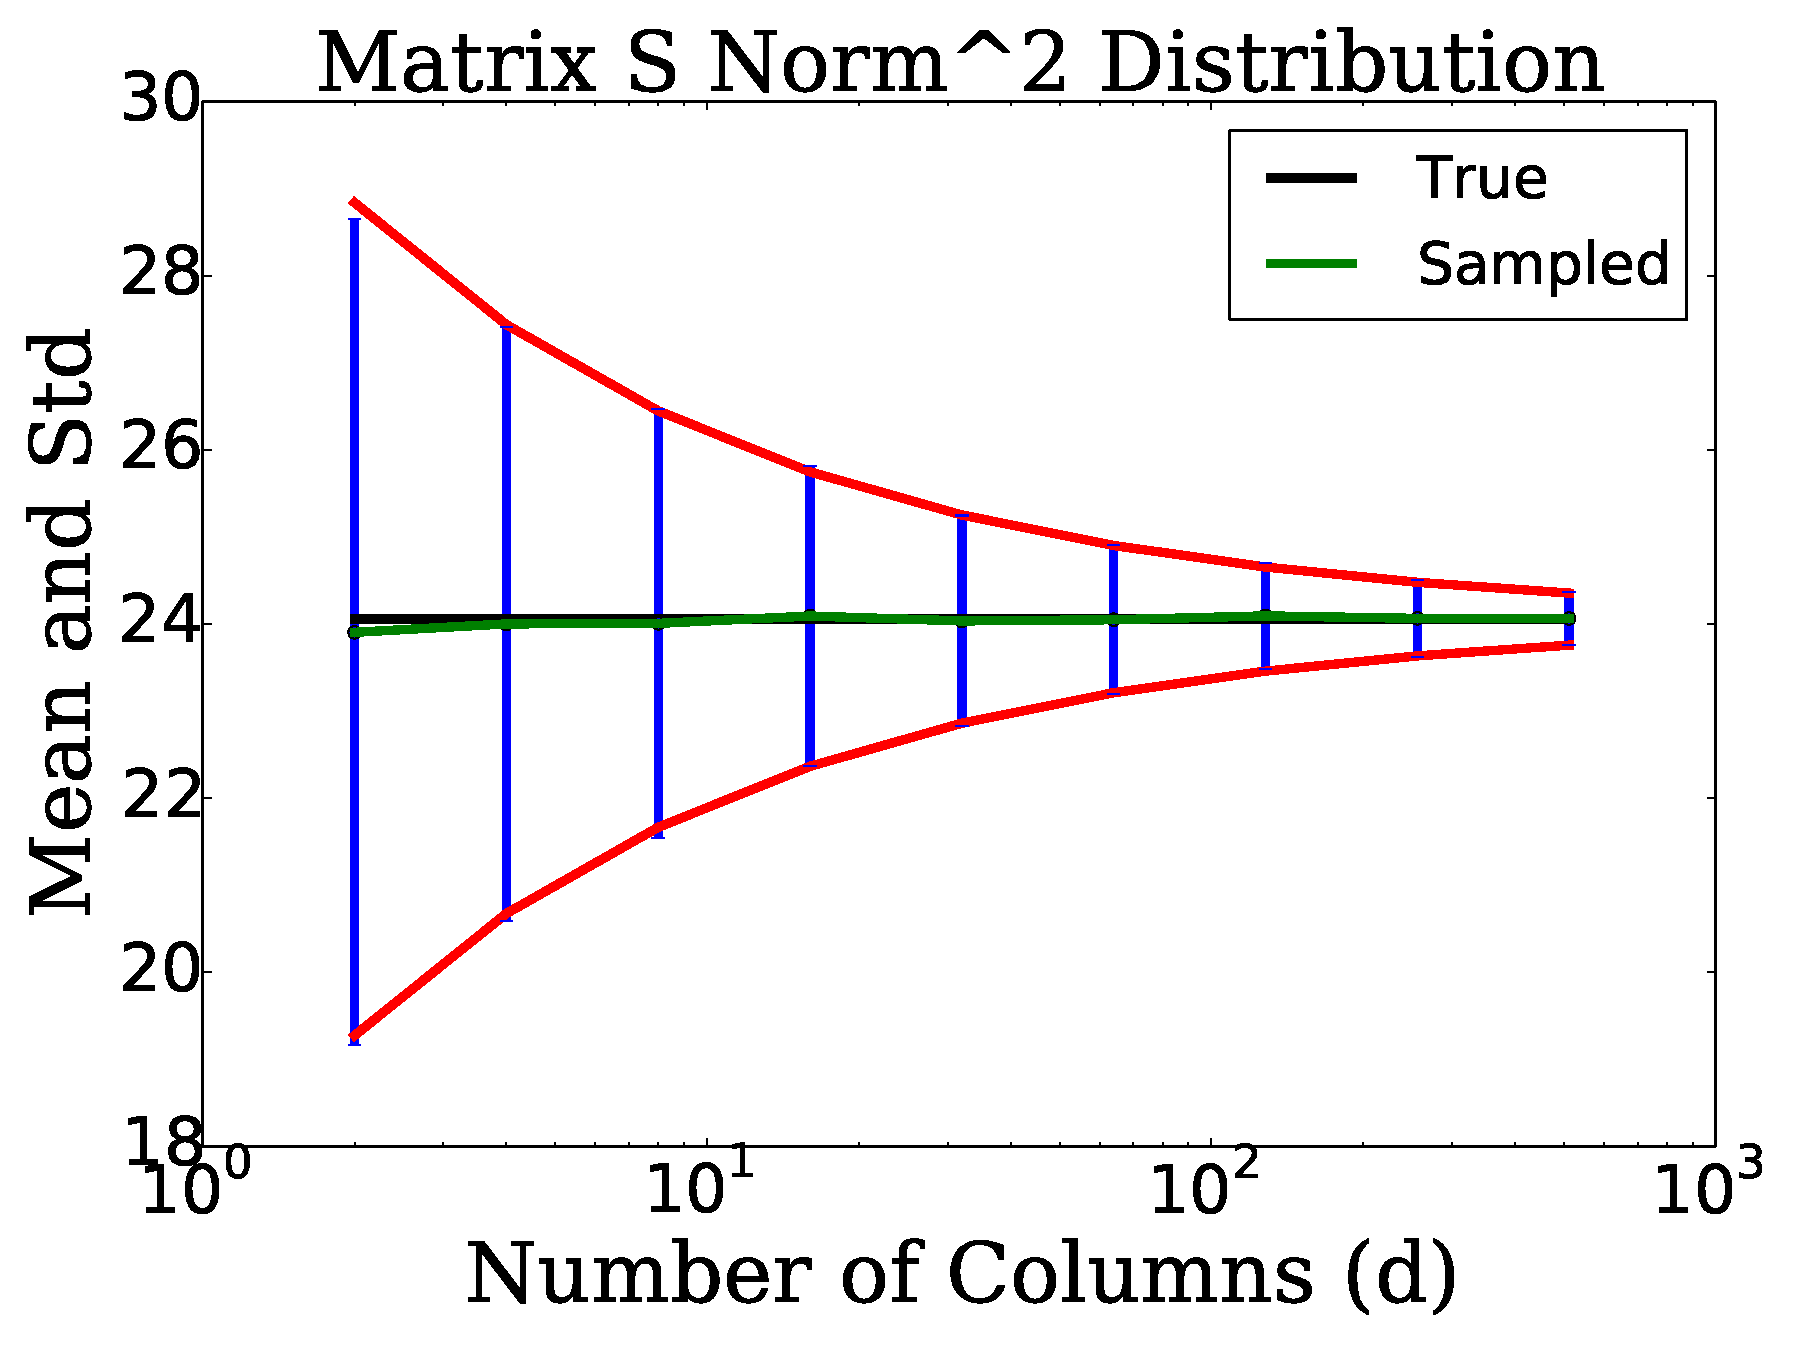
\includegraphics[width=\textwidth]{plots/mat_S_error_test_2.pdf}
    \caption{Matrix S}
    \end{subfigure}
    \begin{subfigure}{0.45\textwidth}
    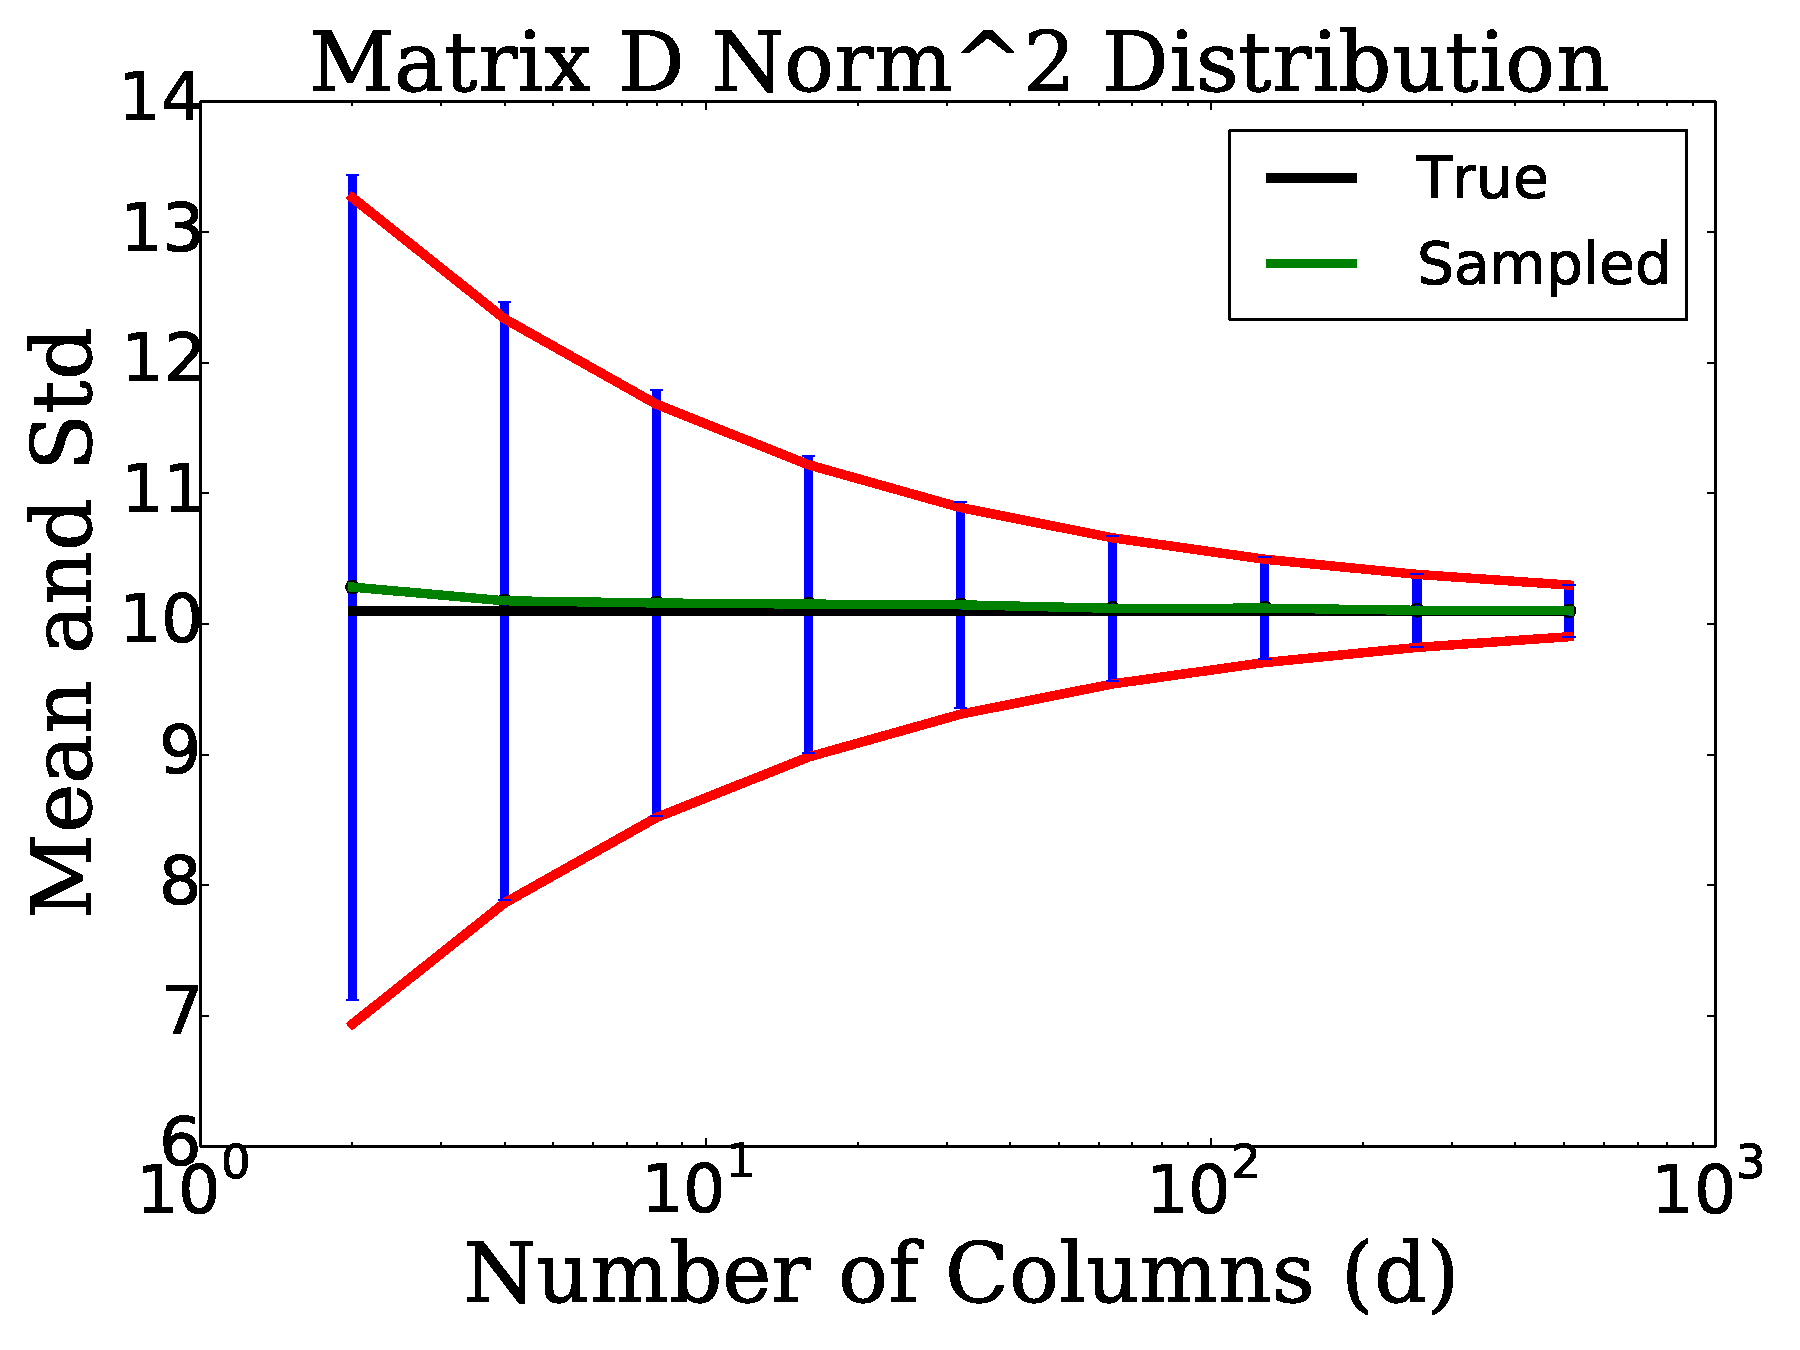
\includegraphics[width=\textwidth]{plots/mat_D_error_test_2.pdf}
    \caption{Matrix D}
    \end{subfigure}

\caption[GEB Stochastic Squared F-norm Approximations]{
%Estimated $||A||_{F}$ for our matrices using the Gaussian Error Bound.
We performed 10,000 trials and computed the
mean (Green) and standard deviation (Blue) of $\norm{A\Omega}_{F}^{2}$
for columns $d\in\{2,4,8,\cdots,512\}$.
The true squared F-norm value is Black and the theoretical standard
deviation bounds from Eq.~\eqref{eq:rand_Xd_variance_bounds} are Red.
}
\label{fig:geb_norm_squared_bound_mat}
\end{figure}






\subsection{Adaptive Comparison}

We now compare some of the adaptive low-rank algorithms;
in particular, we use Alg.~\ref{alg:rand_low_rank} with the HMT
stopping criterion, the YGL algorithm in Alg.~\ref{alg:rand_low_rank_YGL},
and the new randomized low-rank compression algorithm
in Alg.~\ref{alg:rand_new_low_rank}.
Once each algorithm has determined enough random samples have been computed,
a pivoted QR factorization is computed on the entire batch
and the factorization is truncated below the specified tolerance.
This last part (pivoted QR) is not an explicit feature of
Algs.~\ref{alg:rand_low_rank}--\ref{alg:rand_low_rank_YGL} but is added
due to it being necessary in the situation where our new algorithm
was developed~\cite{randomHSSLBL}.
These results can be found in Table~\ref{tab:results_qb_approx_mat};
the minimum samples required to meet the specified tolerance
(as determined by the SVD) are given in Table~\ref{tab:results_qb_min_rank}.
The averaged number of random samples used is computed as well
as the average 2-norm error taken over 1,000 trials.
While the YGL and new algorithm bounds are related to the F-norm,
the 2-norm is of primary importance.
Random samples are computed in blocks of 16 random samples and,
due to the nature of our new algorithm, the minimum possible number of
samples used in Alg.~\ref{alg:rand_new_low_rank} is 32:
16 samples for initial $Q$ and 16 samples for the error estimate.
The YGL algorithm stops if we compute $E\le0$.

From the results, we see that the HMT bound always performs the worst
in every case; this is expected from it overestimating the 2-norm.
Outside of this, the YGL and GEB algorithms are close.
Matrix A1 is particularly challenging: it has slow singular value decay
and our algorithm performs no power iteration.
For this matrix, YGL does better than GEB in every case
(they perform equally well with a relative error of $0.1$), in part
because knowing the error exactly is important.
For Matrix A2, YGL does better for $0.1$ relative error, with GEB
using fewer or equal samples in the other cases.
Matrices E1, E2, and S are similar: YGL and GEB are about the same
for large relative errors but, due to the inherent error bound restrictions,
the new algorithm is better for smaller tolerances.
For Matrix D, YGL did a little better than GEB.
Overall, the results here show that the YGL stopping criterion
may be slightly better than the GEB stopping criterion when
for $\epsr\ge O(\sqrt{\epsm})$, but our stochastic F-norm bound allows us
to determine relative errors to smaller tolerances.

We now perform more runs, except here we only look at the new
stopping criterion;
we set the blocksize to 5 and change the relative tolerances.
Results are shown in Table~\ref{tab:results_qb_approx_mat_geb_hard},
and Table~\ref{tab:results_qb_min_rank_tough_geb} contains the minimum
required ranks.
The relative tolerances here are difficult and are meant to test
the limits of our stopping criterion.
For Matrix E1, we are able to have relative tolerances down to
5E-15 without having any problems with the
stopping criterion (that is, every trial determined 100 samples
was sufficient for the specified tolerance);
some trials failed to satisfy the stopping criterion for 1E-15 and
no trials satisfied the stopping criterion for 5E-16.
These difficulties are expected because we are getting close to
the limitations of machine precision ($\epsm\approx10^{-16}$
for double precision).
For Matrix S, we note that we use an average of 107 samples for
the tolerance 1E-14, which is more than the 100 samples that
should be sufficient ideally.
For Matrix D, we used \textbf{single precision}.
We did not have any problems with relative tolerances down
to 5E-6; for the tolerance 1E-6, most trials (738/1000) failed to
satisfy the stopping criterion.
Again, this is expected because $\epsm\approx10^{-7}$ in single precision.
Overall, we see that our new stopping criterion allows us to get
close to machine precision, which is not the case
when using the HMT or YGL algorithms.

%%%%%%%%%%%%%%%%%%%%%%%%%%%%%%%%%%%%%%%%%%%%%%%%%%%%%%%%%%%%%%%%%%%%%%%%
%%% HMT/YGL/GEB QB Approx table

\begin{table}
\begin{center}
\begin{tabular}{|c|c|c|c|c|c|c|c|c|}
\cline{2-9}
\multicolumn{1}{c|}{} &
\multicolumn{2}{|c|}{\textbf{0.75}} & \multicolumn{2}{|c|}{\textbf{0.5}} &
\multicolumn{2}{|c|}{\textbf{0.25}} & \multicolumn{2}{|c|}{\textbf{0.1}} \\
\hline
Matrix A1 &
Err & Samp & Err & Samp &
Err & Samp & Err & Samp \\
\hline
HMT & 0.19 & 128 & 0.16 & 128 & 0.13 & 128 & 3E-15 & 128 \\
\hline
YGL & 0.45 & 20 & 0.24 & 59 & 0.16 &  96 & 3E-3 & 112 \\
\hline
GEB & 0.22 & 77 & 0.18 & 94 & 0.15 &  102 & 5E-3 & 112 \\
\hline
\hline
\multicolumn{1}{c|}{} &
\multicolumn{2}{|c|}{\textbf{1E-1}} & \multicolumn{2}{|c|}{\textbf{1E-2}} &
\multicolumn{2}{|c|}{\textbf{1E-3}} & \multicolumn{2}{|c|}{\textbf{1E-4}} \\
\hline
Matrix A2 &
Err & Samp & Err & Samp &
Err & Samp & Err & Samp \\
\hline
HMT & 4E-2 & 42 & 3E-3 & 92 & 3E-4 & 128 & 2E-15 & 128 \\
\hline
YGL & 4E-2 & 16 & 5E-3 & 32 & 4E-4 &  96 & 2E-15 & 112 \\
\hline
GEB & 4E-2 & 32 & 5E-3 & 32 & 4E-4 &  80 & 2E-15 & 112 \\
\hline
\hline
\multicolumn{1}{c|}{} &
\multicolumn{2}{|c|}{\textbf{1E-3}} & \multicolumn{2}{|c|}{\textbf{1E-6}} &
\multicolumn{2}{|c|}{\textbf{1E-9}} & \multicolumn{2}{|c|}{\textbf{1E-12}} \\
\hline
Matrix E1 &
Err & Samp & Err & Samp &
Err & Samp & Err & Samp \\
\hline
HMT & 4E-4 & 48 & 4E-7 & 76 & 4E-10 & 96 & 4E-13 & 112 \\
\hline
YGL & 6E-4 & 32 & 7E-7 & 48 & 1E-9  & 64 & 6E-10 & 64 \\
\hline
GEB & 6E-4 & 32 & 7E-7 & 48 & 1E-9  & 65 & 7E-13 & 94 \\
\hline
\hline
\multicolumn{1}{c|}{} &
\multicolumn{2}{|c|}{\textbf{1E-3}} & \multicolumn{2}{|c|}{\textbf{1E-6}} &
\multicolumn{2}{|c|}{\textbf{1E-9}} & \multicolumn{2}{|c|}{\textbf{1E-12}} \\
\hline
Matrix E2 &
Err & Samp & Err & Samp &
Err & Samp & Err & Samp \\
\hline
HMT & 3E-4 & 32 & 3E-7 & 48 & 4E-10 & 53 & 3E-13 & 82* \\
\hline
YGL & 6E-4 & 16 & 4E-7 & 32 & 8E-10 & 32 & 1E-10 & 32 \\
\hline
GEB & 3E-4 & 32 & 4E-7 & 32 & 8E-10 & 32 & 5E-13 & 48 \\
\hline
\hline
\multicolumn{1}{c|}{} &
\multicolumn{2}{|c|}{\textbf{1E-3}} & \multicolumn{2}{|c|}{\textbf{1E-6}} &
\multicolumn{2}{|c|}{\textbf{1E-9}} & \multicolumn{2}{|c|}{\textbf{1E-12}} \\
\hline
Matrix S &
Err & Samp & Err & Samp &
Err & Samp & Err & Samp \\
\hline
HMT & 4E-4 & 64 & 3E-7 & 80 & 4E-10 & 80 & 3E-13 & 200+ \\
\hline
YGL & 5E-4 & 48 & 2E-6 & 48 & 6E-10 & 64 & 2E-11 & 64 \\
\hline
GEB & 5E-4 & 48 & 9E-7 & 59 & 6E-10 & 64 & 6E-13 & 80 \\
\hline
\hline
\multicolumn{1}{c|}{} &
\multicolumn{2}{|c|}{\textbf{1E-1}} & \multicolumn{2}{|c|}{\textbf{1E-3}} &
\multicolumn{2}{|c|}{\textbf{1E-5}} & \multicolumn{2}{|c|}{\textbf{1E-7}} \\
\hline
Matrix D &
Err & Samp & Err & Samp &
Err & Samp & Err & Samp \\
\hline
HMT & 3E-2 & 51 & 4E-4 & 80 & 4E-6 & 96 & 4E-8 & 112 \\
\hline
YGL & 9E-2 & 27 & 6E-4 & 48 & 1E-5 & 64 & 2E-7 & 85 \\
\hline
GEB & 5E-2 & 32 & 6E-4 & 48 & 9E-6 & 69 & 6E-8 & 96 \\
\hline
\end{tabular}
\end{center}
\caption[QB Adaptive Approximation Results]{
QB approximation results for Matrices A1, A2, E1, E2, S, and D.
For each absolute error tolerance, we averaged 1,000 trials to determine
the average error (Err) and average samples used (Samp) in order to compute
a QB approximation once we used either the HMT stopping criterion,
the YGL stopping criterion, or the new stopping criterion to
determine when we had approximated the range.
Random samples were computed in blocks of 16.
In the case when we used $200+$ samples,
we were not able to meet the HMT stopping criterion
and used the maximum of 200 random samples.
Some of the data here was originally in~\cite{randomHSSLBL}.
The minimum possible ranks can be found in Table~\ref{tab:results_qb_min_rank}.
A ``*'' means that there were some runs which reached the maximum allowable
samples of 200 before compression.
}
\label{tab:results_qb_approx_mat}
\end{table}

%%%%%%%%%%%%%%%%%%%%%%%%%%%%%%%%%%%%%%%%%%%%%%%%%%%%%%%%%%%%%%%%%%%%%%%%
%%% HMT/YGL/GEB QB Approx table

\begin{table}
\begin{center}
\begin{tabular}{|c|c|c|c|c|}
\hline
Matrix A1 & \textbf{0.75} & \textbf{0.5} & \textbf{0.25} & \textbf{0.1} \\
\hline
Min Rank  & 1 & 4 & 16 & 100 \\
\hline
\hline
Matrix A2 & \textbf{1E-1} & \textbf{1E-2} & \textbf{1E-3} & \textbf{1E-4} \\
\hline
Min Rank  & 3 & 10 & 31 & 100 \\
\hline
\hline
Matrix E1 & \textbf{1E-3} & \textbf{1E-6} & \textbf{1E-9} & \textbf{1E-12} \\
\hline
Min Rank  & 19 & 38 & 57 & 76 \\
\hline
\hline
Matrix E2 & \textbf{1E-3} & \textbf{1E-6} & \textbf{1E-9} & \textbf{1E-12} \\
\hline
Min Rank  & 9 & 18 & 27 & 36 \\
\hline
\hline
Matrix S  & \textbf{1E-3} & \textbf{1E-6} & \textbf{1E-9} & \textbf{1E-12} \\
\hline
Min Rank  & 35 & 45 & 55 & 65 \\
\hline
\hline
Matrix D  & \textbf{1E-1} & \textbf{1E-3} & \textbf{1E-5} & \textbf{1E-7} \\
\hline
Min Rank  & 20 & 40 & 60 & 80 \\
\hline
\hline
\end{tabular}
\end{center}
\caption[QB Adaptive Test: Minimum Rank]{
Here are the absolute minimum ranks required
for Matrices A1, A2, E1, E2, S, and D.
}
\label{tab:results_qb_min_rank}
\end{table}


%%%%%%%%%%%%%%%%%%%%%%%%%%%%%%%%%%%%%%%%%%%%%%%%%%%%%%%%%%%%%%%%%%%%%%%%
%%% HMT/YGL/GEB QB Approx table

\begin{table}
\begin{center}
\begin{tabular}{|c|c|c|c|c|c|c|c|c|}
\cline{2-9}
\multicolumn{1}{c|}{} &
\multicolumn{2}{|c|}{\textbf{1E-14}} & \multicolumn{2}{|c|}{\textbf{5E-15}} &
\multicolumn{2}{|c|}{\textbf{1E-15}} & \multicolumn{2}{|c|}{\textbf{5E-16}} \\
\hline
Matrix E1 &
Err & Samp & Err & Samp &
Err & Samp & Err & Samp \\
\hline
GEB & 1E-14 & 97 & 4E-15 & 100 & 6E-16  & 144* & 7E-16 & 200+ \\
\hline
\hline
\multicolumn{1}{c|}{} &
\multicolumn{2}{|c|}{\textbf{5E-13}} & \multicolumn{2}{|c|}{\textbf{1E-13}} &
\multicolumn{2}{|c|}{\textbf{4E-14}} & \multicolumn{2}{|c|}{\textbf{1E-14}} \\
\hline
Matrix S &
Err & Samp & Err & Samp &
Err & Samp & Err & Samp \\
\hline
GEB & 4E-13 & 75 & 7E-14 & 96 & 5E-14 & 100 & 9E-15 & 107 \\
\hline
\hline
\multicolumn{1}{c|}{} &
\multicolumn{2}{|c|}{\textbf{5E-5}} & \multicolumn{2}{|c|}{\textbf{1E-5}} &
\multicolumn{2}{|c|}{\textbf{5E-6}} & \multicolumn{2}{|c|}{\textbf{1E-6}} \\
\hline
Matrix D &
Err & Samp & Err & Samp &
Err & Samp & Err & Samp \\
\hline
GEB (s) & 4E-5 & 59 & 9E-6 & 66 & 9E-6 & 71 & 6E-7 & 186* \\
\hline
\end{tabular}
\end{center}
\caption[QB Adaptive Approximation Results (Stringent GEB Tests)]{
Tough QB approximation results for Matrices E1, S, and D
using the new GEB stopping criterion.
For each absolute error tolerance, we averaged 1,000 trials to determine
the average error (Err) and average samples used (Samp) in order to compute
a QB approximation once we used the new stopping criterion to
determine when we had approximated the range.
Random samples were computed in blocks of 5.
For matrix D, we used \textbf{single precision}.
In the case when we used $200+$ samples,
we were not able to meet the HMT stopping criterion
and used the maximum of 200 random samples.
The minimum possible ranks can be found in
Table~\ref{tab:results_qb_min_rank_tough_geb}.
A ``*'' means that there were some runs which reached the maximum allowable
samples of 200 before compression.
For matrix E1 with $\epsr$=1E-15, 7.7\% of the trials used over 200 samples
(and so failed to stop);
for matrix D  with $\epsr$=1F-6, 73.8\% of the trials used over 200 samples.
}
\label{tab:results_qb_approx_mat_geb_hard}
\end{table}

%%%%%%%%%%%%%%%%%%%%%%%%%%%%%%%%%%%%%%%%%%%%%%%%%%%%%%%%%%%%%%%%%%%%%%%%
%%% HMT/YGL/GEB QB Approx table

\begin{table}
\begin{center}
\begin{tabular}{|c|c|c|c|c|}
\hline
Matrix E1 & \textbf{1E-14} & \textbf{5E-15} & \textbf{1E-15} & \textbf{5E-16} \\
\hline
Min Rank  & 88 & 90 & 95 & 96 \\
\hline
\hline
Matrix S  & \textbf{5E-13} & \textbf{1E-13} & \textbf{5E-14} & \textbf{1E-14} \\
\hline
Min Rank  & 66 & 69 & 71 & 100 \\
\hline
\hline
Matrix D  & \textbf{5E-5} & \textbf{1E-5} & \textbf{5E-6} & \textbf{1E-6} \\
\hline
Min Rank  & 50 & 60 & 60 & 70 \\
\hline
\hline
\end{tabular}
\end{center}
\caption[QB Adaptive Test: Minimum Rank (Stringent GEB Test)]{
Here are the absolute minimum ranks required for Matrices E1, S, and D.
}
\label{tab:results_qb_min_rank_tough_geb}
\end{table}




\subsection{Stopping Criteria Discussion}

The results of this section show our new stopping criterion does well,
usually being on par or better than other stopping criteria
while allowing for small tolerances.
One noticeable difficultly, shared by others, is using too many
additional samples to perform a low-order approximation
($\epsr\gtrsim0.1$) for matrices with slow decay without using power iteration;
part of the difficulty comes from using F-norm
bounds when desiring 2-norm accuracy.
Outside of this limited range, the error closely matches
the specified tolerance, keeping communication-heavy computations
to one rank-revealing QR factorization.
Additionally, we showed our stopping criterion
allows us to approximate matrices to relative tolerances
close to machine precision.
